\documentclass{article}
\usepackage{graphicx} % Required for inserting images
\usepackage [utf8]{ctex}
\usepackage{listings}

\title{Data Ingestion Tools}
\author{211870287 丁旭 }
\date{September 2023}

\begin{document}

\maketitle

\section{任务一 使用 Apache Kafka 进行数据流}
\begin{enumerate}
    \item 预置安装Zookeeper-3.9.0
    \begin{lstlisting}
0、下载zookeeper
wget https://mirrors.tuna.tsinghua.edu.cn/apache/zookeeper/zookeeper-3.9.0/apache-zookeeper-3.9.0-bin.tar.gz --no-check-certificate

1、解压到/usr/local/目录下
tar -zxvf ./apache-zookeeper-3.9.0-bin.tar.gz -C /usr/local/

2、进入目录并修改名称
cd /usr/local && mv apache-zookeeper-3.9.0-bin/ zookeeper-3.9.0

3、进入 zookeeper 创建两个文件
cd zookeeper-3.9.0
mkdir data 
mkdir logs

4、创建配置文件
vim conf/zoo.cfg

5、写入配置信息
tickTime = 2000
dataDir = /usr/local/zookeeper-3.9.0/data
dataLogDir = /usr/local/zookeeper-3.9.0/logs
tickTime = 2000
clientPort = 2181
initLimit = 5
syncLimit = 2

启动zookeeper
启动服务:
/usr/local/zookeeper-3.9.0/bin/zkServer.sh start

连接服务:
/usr/local/zookeeper-3.9.0/bin/zkCli.sh

查看服务状态:
/usr/local/zookeeper-3.9.0/bin/zkServer.sh status

停止服务:
/usr/local/zookeeper-3.9.0/bin/zkServer.sh stop
    \end{lstlisting}
    \begin{figure}[htp]
        \centering
        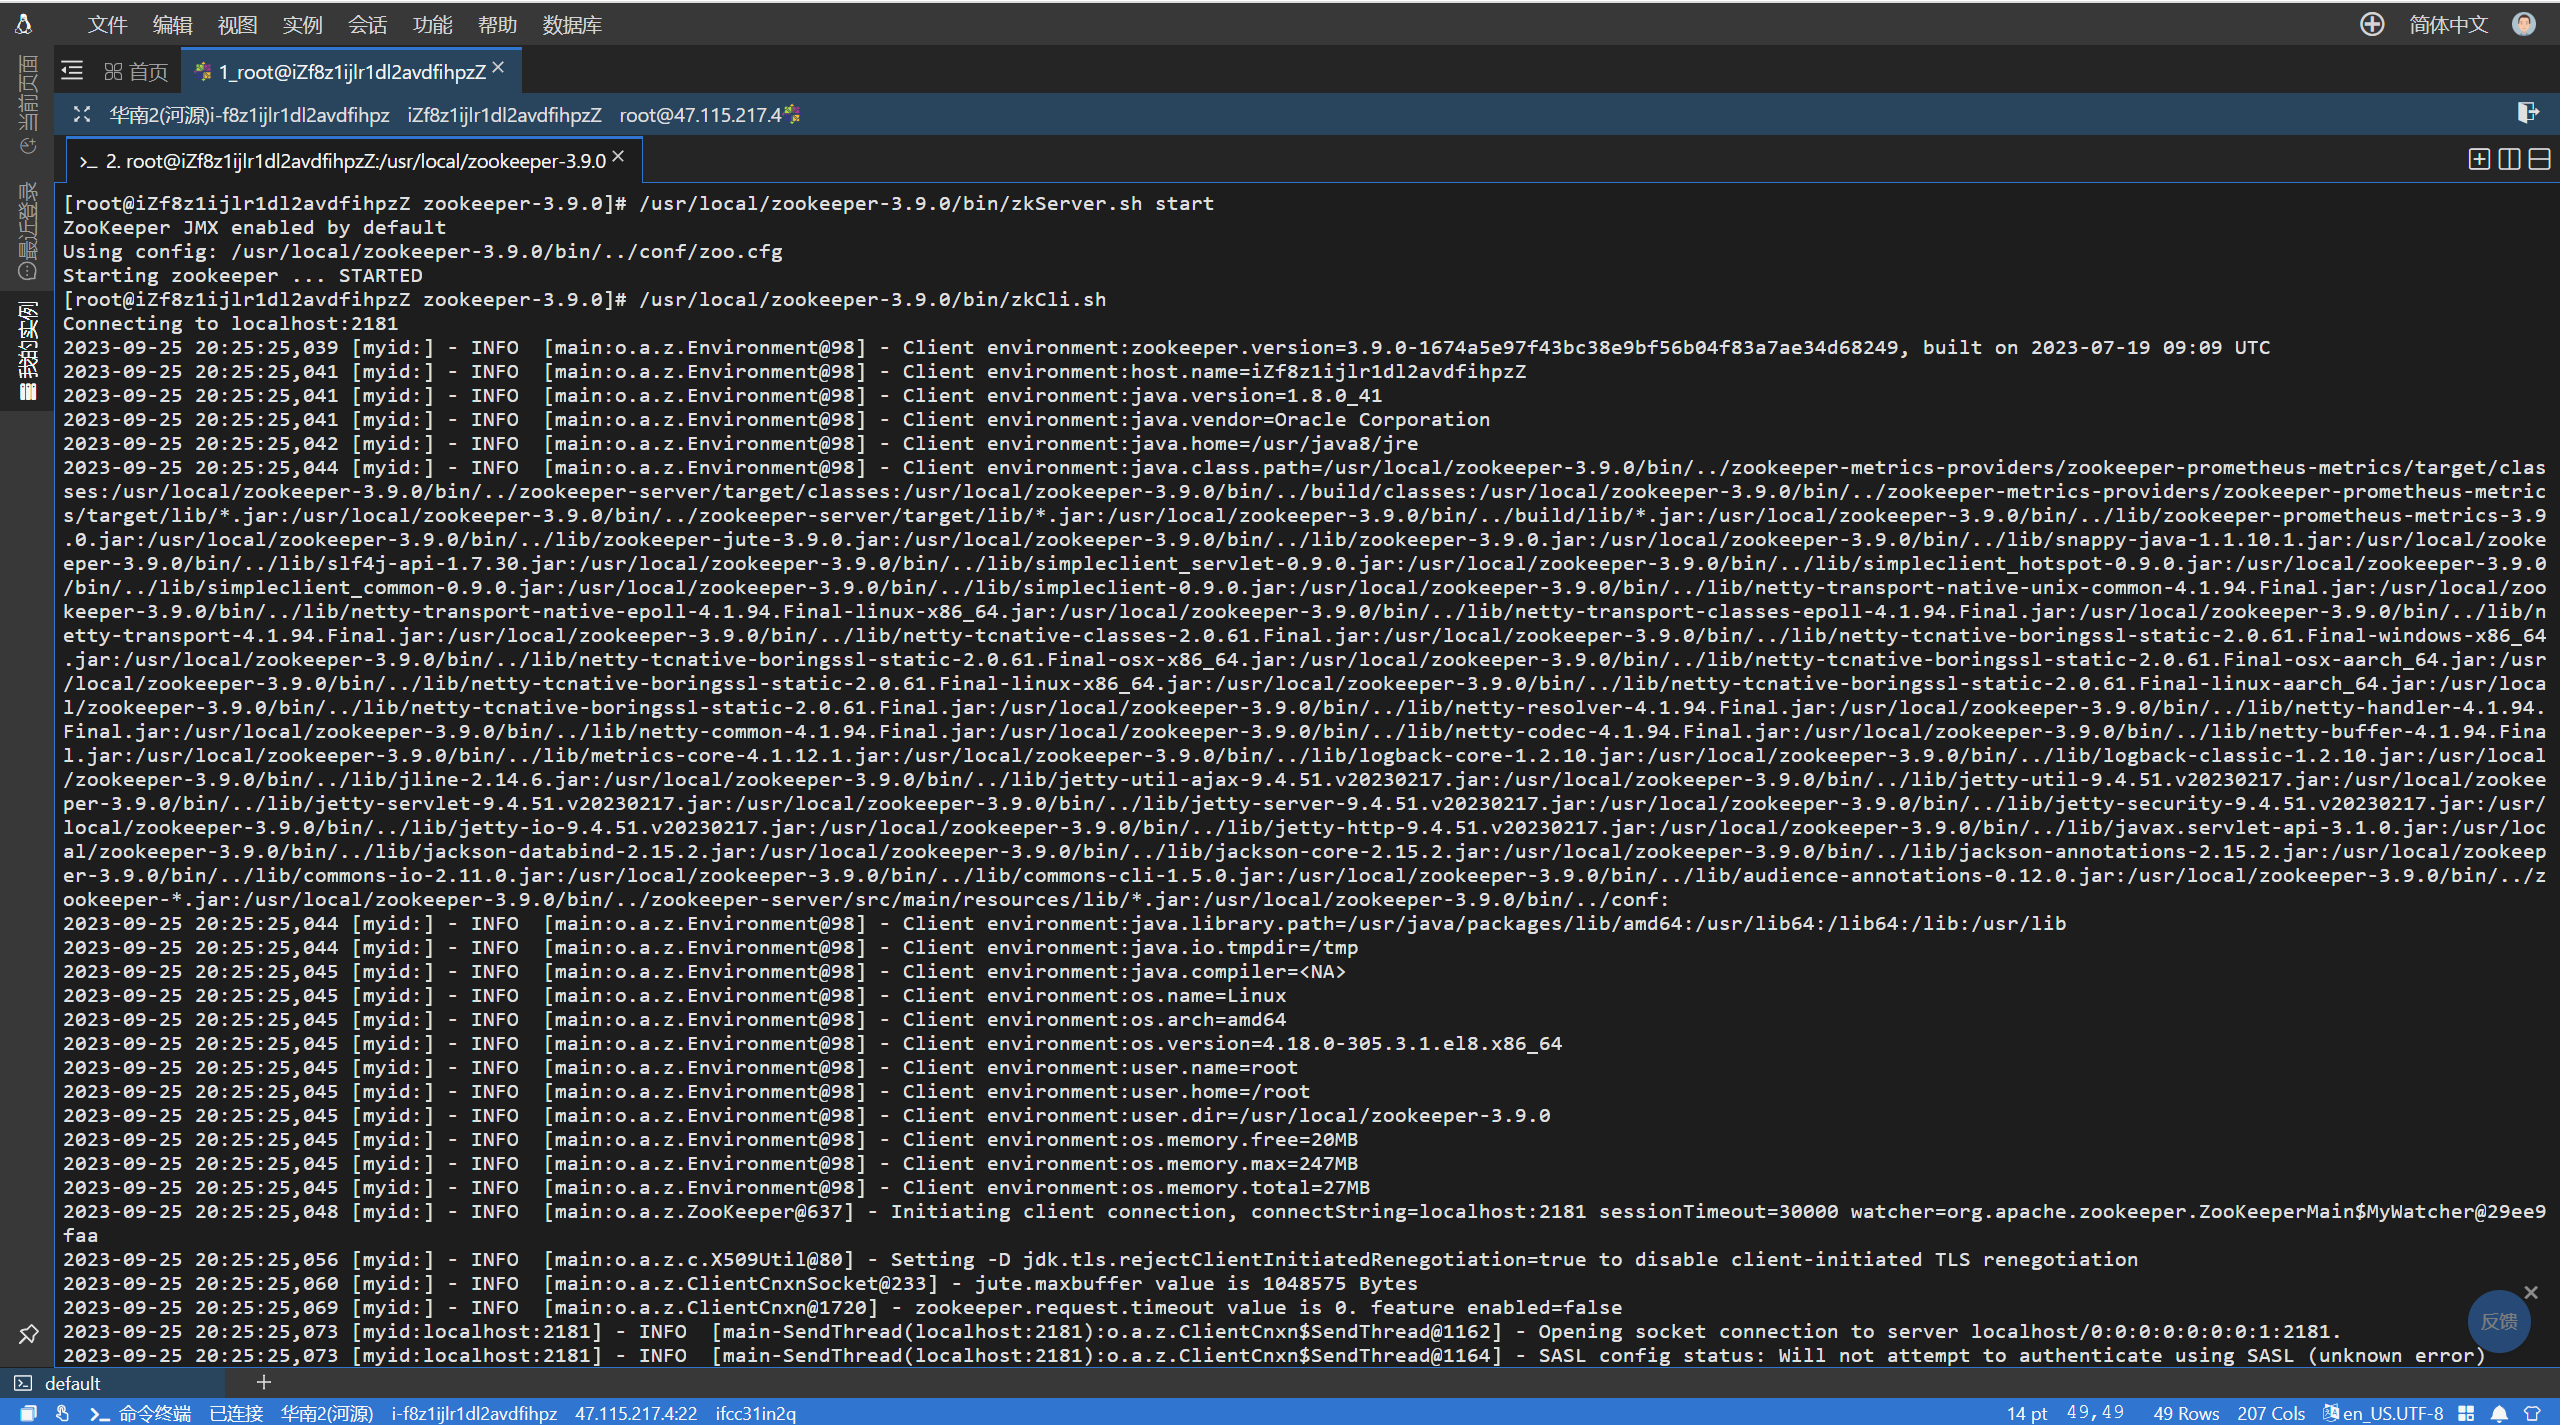
\includegraphics[width=13cm]{zookeeper启动.png}
        \caption{zookeeper启动}
        \label{pic1}
    \end{figure}
    \newpage
    \begin{figure}[htp]
        \centering
        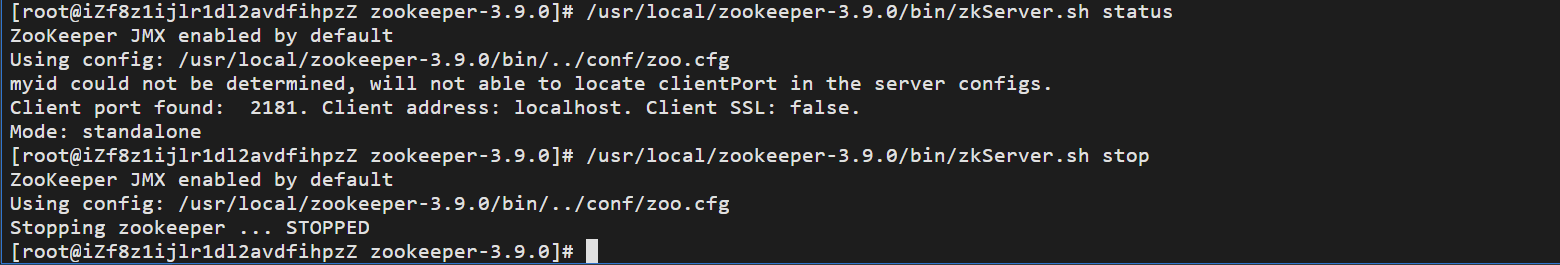
\includegraphics[width=15cm]{zookeeper_status.png}
        \caption{zookeeper status命令}
        \label{pic2}
    \end{figure}
    \begin{figure}[htp]
        \centering
        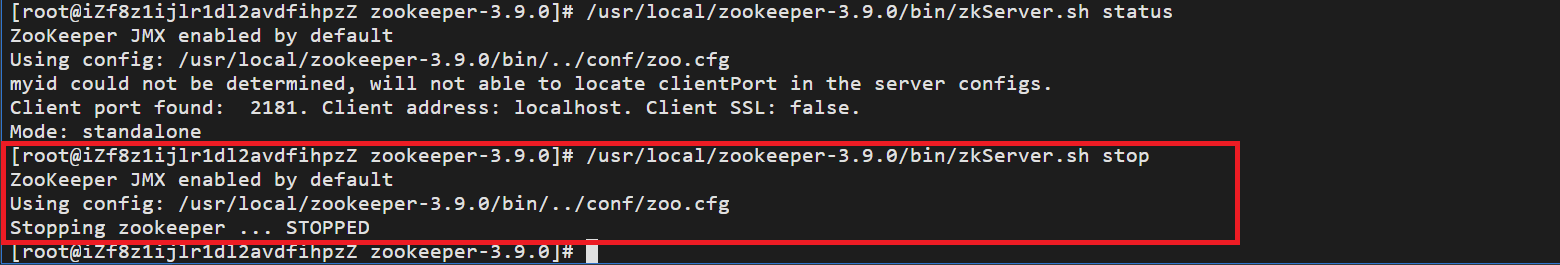
\includegraphics[width=15cm]{zookeeper_stop.png}
        \caption{zookeeper stop命令}
        \label{pic3}
    \end{figure}
    \item 安装Kafka
    \begin{lstlisting}
0、linux中使用wget命令,远程下载kafka
wget https://archive.apache.org/dist/kafka/2.8.1/kafka_2.12-2.8.1.tgz  --no-check-certificate

1、解压压缩包到/usr/local/目录
tar -zxvf ./kafka_2.12-2.8.1.tgz -C /usr/local/

2、进入/usr/local/目录
cd /usr/local/

3、修改原始名称
mv ./kafka_2.12-2.8.1/ kafka2.12

4、进入Kafka并修改配置文件
cd kafka2.12
vim config/server.properties

修改其中的:
broker.id=1
log.dir=/usr/local/kafka/kafka-logs

#配置kafka的监听端口
listeners=PLAINTEXT://:9092

#把kafka的地址端口注册给zookeeper,如果是远程访问要改成外网IP
advertised.listeners=PLAINTEXT://:9092

————————————————————

kafka启动命令(必须先启动zookeeper!):
/usr/local/zookeeper-3.9.0/bin/zkServer.sh start
/usr/local/kafka2.12/bin/kafka-server-start.sh -daemon config/server.properties
注:可以将bin文件路径加到.bashrc中
例: 
export PATH="/usr/local/kafka/bin:$PATH"
source ~/.bashrc
kafka-server-start.sh -daemon config/server.properties

kafka停止命令:
bin/kafka-server-stop.sh
    \end{lstlisting}
    \begin{figure}[htp]
        \centering
        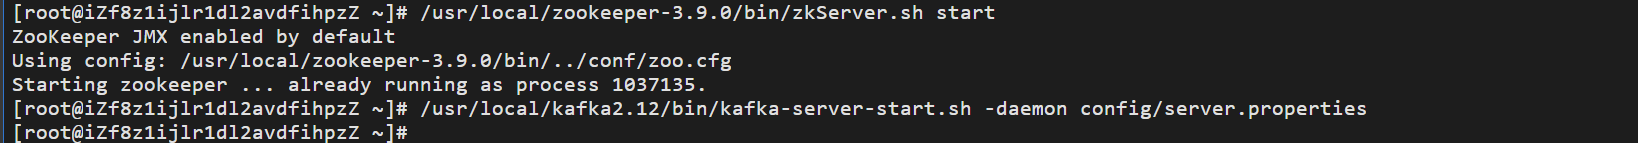
\includegraphics[width=15cm]{kafka_version.png}
        \caption{kafka version命令}
        \label{pic4}
    \end{figure}
    \begin{figure}[htp]
        \centering
        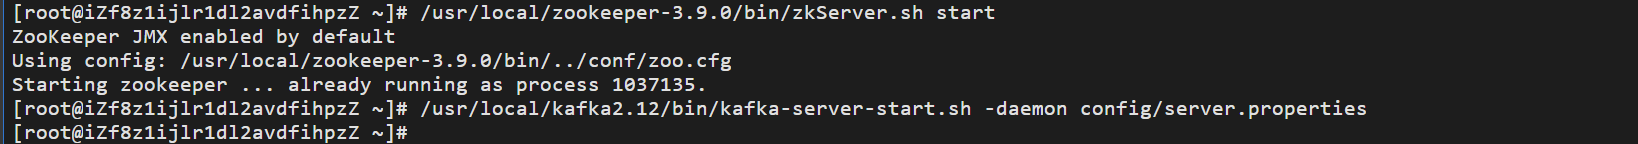
\includegraphics[width=15cm]{kafka_start.png}
        \caption{启动kafka}
        \label{pic5}
    \end{figure}
    \item 生产和消费一个简单的消息。
    \begin{lstlisting}
创建Topic
1、进入到Kafka目录下,创建一个名为testTopic的Topic。
bin/kafka-topics.sh --create --zookeeper localhost:2181 --replication-factor 1 --partitions 1 --topic testTopic

2、查看创建的Topic列表。
bin/kafka-topics.sh --list --zookeeper localhost:2181

测试通信
1、连接生产者,命令后面需要对应 Topic 名称。
bin/kafka-console-producer.sh --broker-list localhost:9092 --topic testTopic
>hhh 
>hello
>actually you are

2连接消费者,需要连接消费者的Topic
bin/kafka-console-consumer.sh --bootstrap-server localhost:9092 --topic testTopic --from-beginning
>hhh
>hello
>actually you are
    \end{lstlisting}
    \begin{figure}[htp]
        \centering
        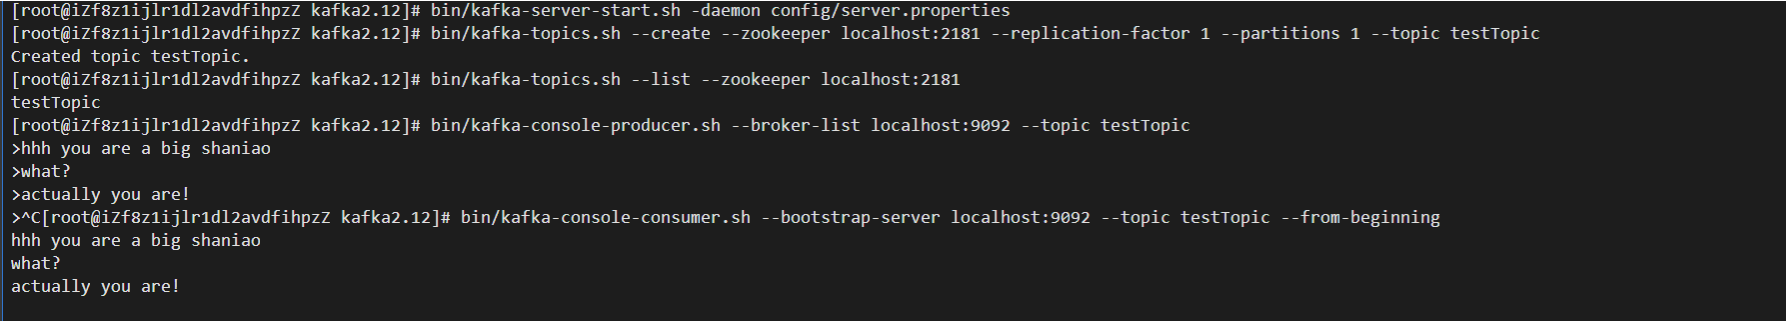
\includegraphics[width=15cm]{test1.png}
        \caption{任务一}
        \label{pic6}
    \end{figure}
    \item 验证
    \par 输入与输出一致,任务完成
\end{enumerate}
\section{任务三 使用 Apache NiFi 进行数据流管理}
\begin{enumerate}
    \item 安装nifi
    \begin{lstlisting}
1. 使用wget 命令 安装nifi (这里我是从清华源安装下载的)
wget https://mirrors.tuna.tsinghua.edu.cn/apache/nifi/1.23.2/nifi-1.23.2-bin.zip

2.解压nifi-1.23.2-bin.tar.gz到/opt/目录下面
tar –zxvf nifi-1.23.2-bin.tar.gz –C /opt/

3.改名nifi
mv nifi-1.23.2-bin nifi

4.配置conf/nifi.properties
https.host: 127.0.0.1
https.port:8443
    \end{lstlisting}
    \begin{figure}[htp]
        \centering
        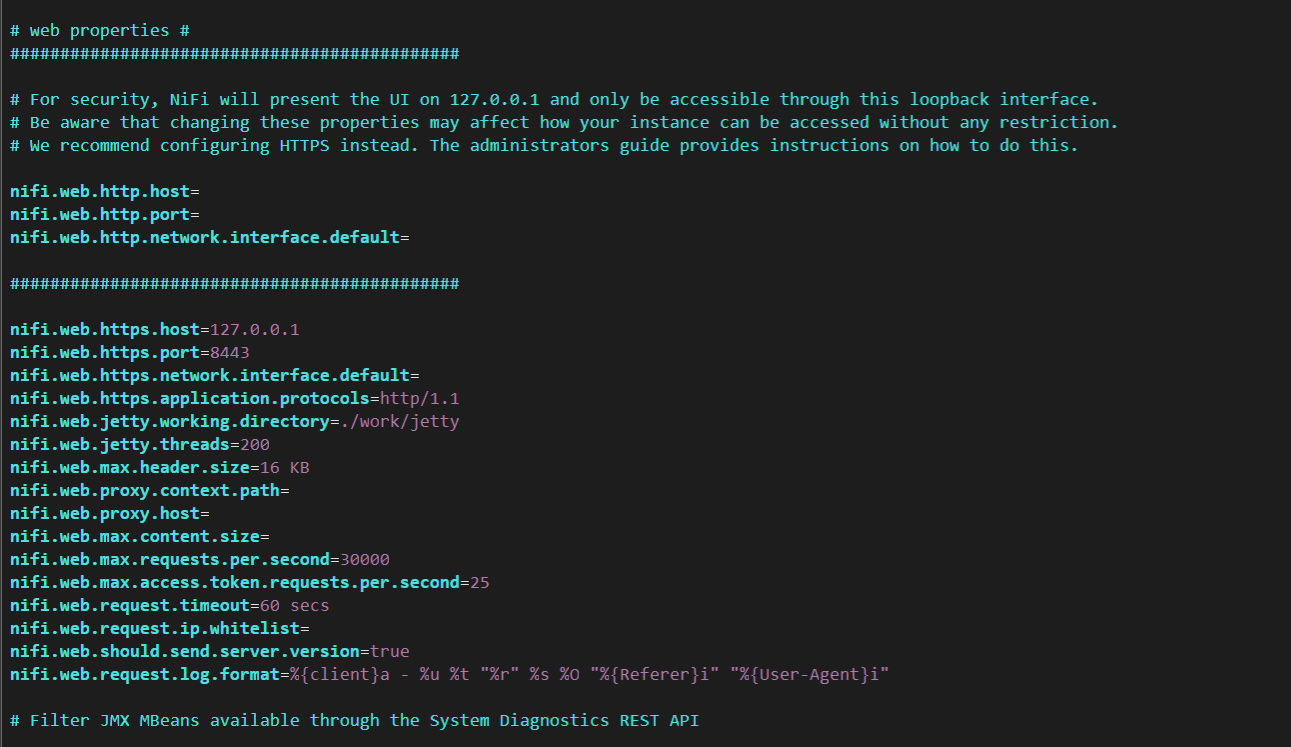
\includegraphics[width=15cm]{nifi_配置.png}
        \caption{conf/nifi.properties}
        \label{pic6}
    \end{figure}
    \begin{lstlisting}
5.运行nifi
nifi.sh start

6.端口映射(因为部署在云服务器的私有ip上 但是不能直接访问网页 需要映射到自己电脑的本地ip上)
这里使用ssh来实现
ssh -i D:/NJU/tmp/nifi.pem -L 8443:localhost:8443 root@47.115.217.4
参数说明:
D:/NJU/tmp/nifi.pem 是存放密钥的路径
8443 映射端口号
root 用户名 
47.115.217.4 公网ip
    \end{lstlisting}
    \begin{figure}[htp]
        \centering
        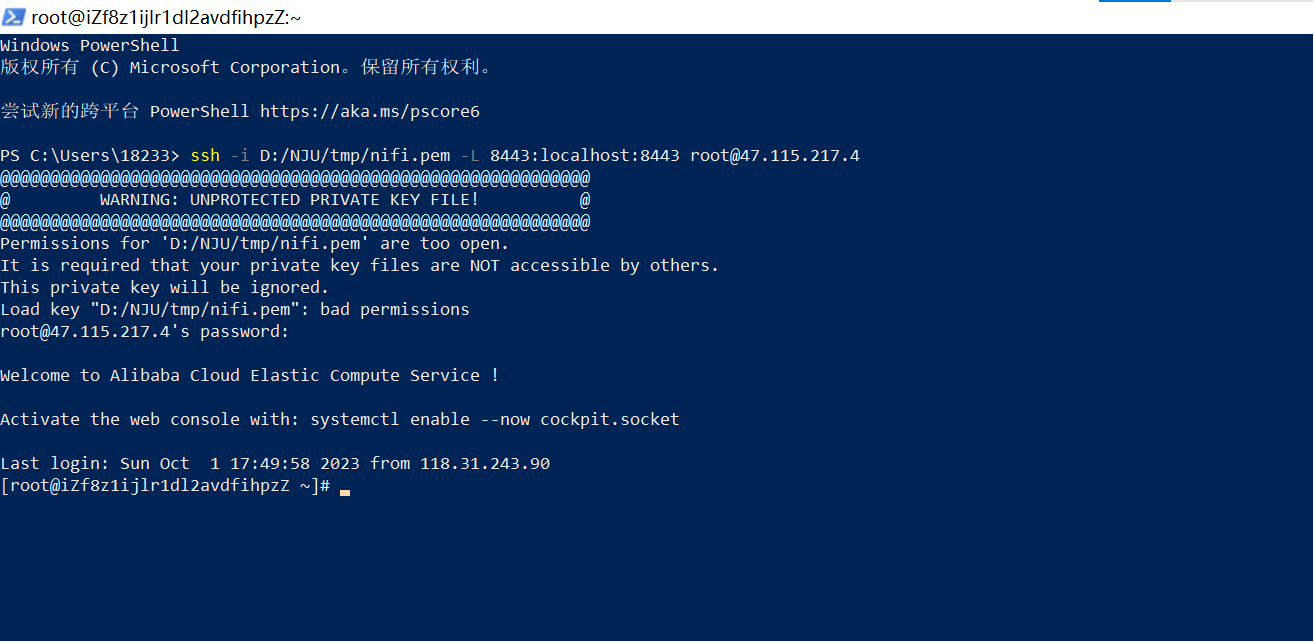
\includegraphics[width=15cm]{端口映射.png}
        \caption{ssh端口映射}
        \label{pic6}
    \end{figure}
    \begin{figure}[htp]
        \centering
        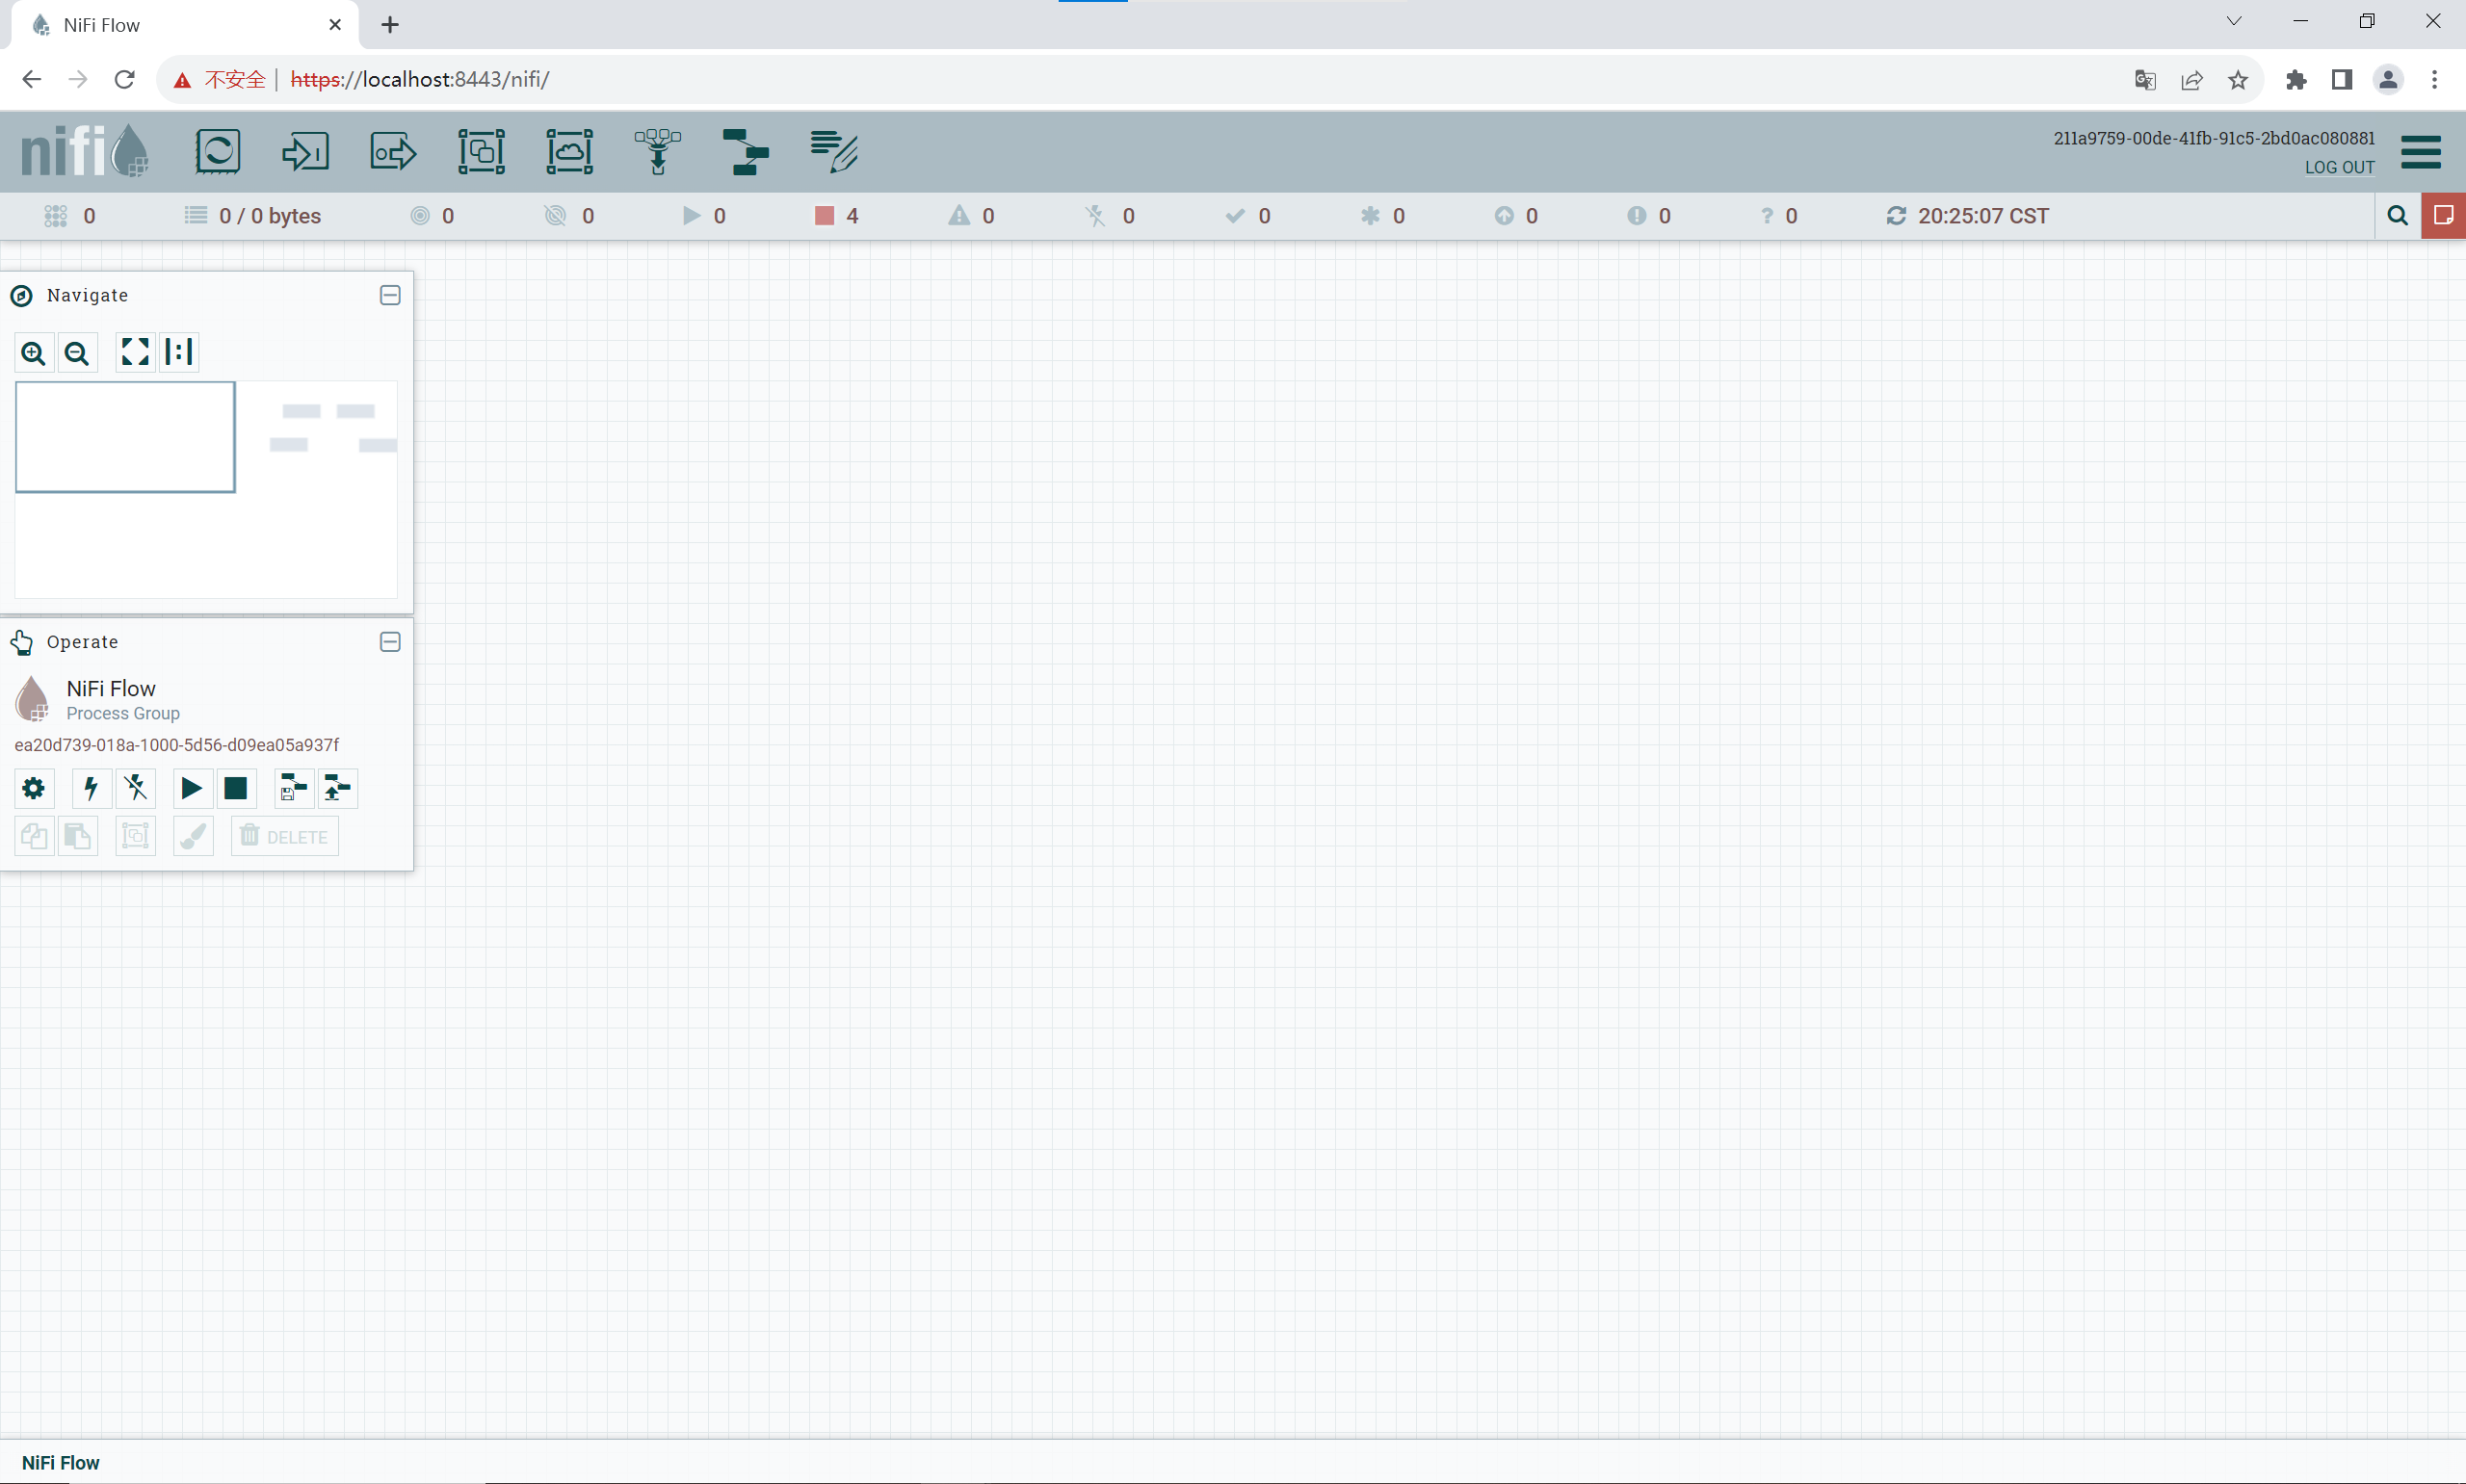
\includegraphics[width=15cm]{进入nifi_web.png}
        \caption{nifi的web界面}
        \label{pic6}
    \end{figure}
    \newpage

    \item 安装mysql
    \begin{lstlisting}
1.下载和安装yum源:
wget https://dev.mysql.com/get/mysql80-community-release-el8-5.noarch.rpm
rpm -ivh mysql80-community-release-el8-5.noarch.rpm

2.安装mysql服务
yum -y install mysql-server
    \end{lstlisting}
    \begin{figure}[htp]
        \centering
        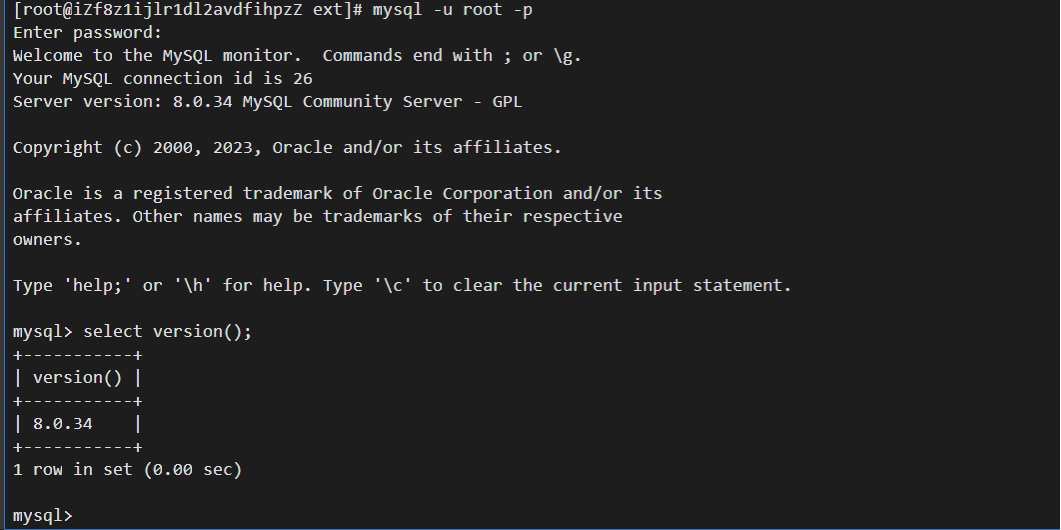
\includegraphics[width=15cm]{mysql_version.png}
        \caption{mysql-version}
        \label{pic6}
    \end{figure}
    \begin{figure}[htp]
        \centering
        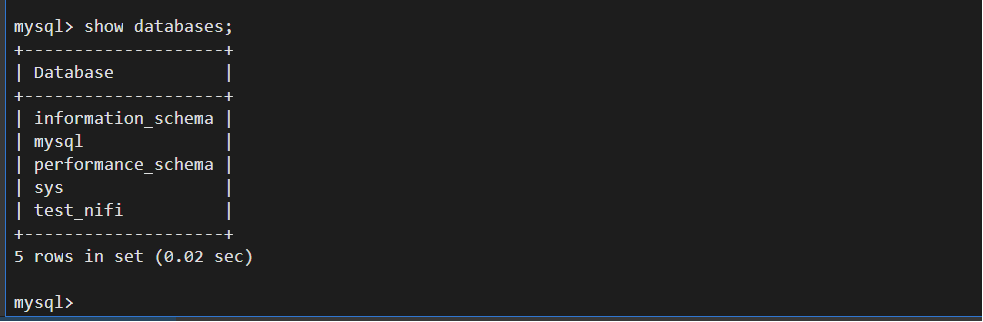
\includegraphics[width=13cm]{创建database.png}
        \caption{database}
        \label{pic6}
    \end{figure}
    \newpage
    
    \item 安装MySQL连接驱动文件mysql-connector-java
    \begin{lstlisting}
1.下载
wget https://downloads.mysql.com/archives/get/p/3/file/mysql-connector-java-8.0.22-1.el7.noarch.rpm    

2.安装依赖
yum -y install java-headless
 
3.安装mysql-connector-java
[root@study1 opt]# rpm -ivh mysql-connector-java-8.0.22-1.el7.noarch.rpm 

4.将mysql-connector-java.jar移至/usr/java8/jre/lib/ext中
mv mysql-connector-java.jar /usr/java8/jre/lib/ext
    \end{lstlisting}
    \begin{figure}[htp]
        \centering
        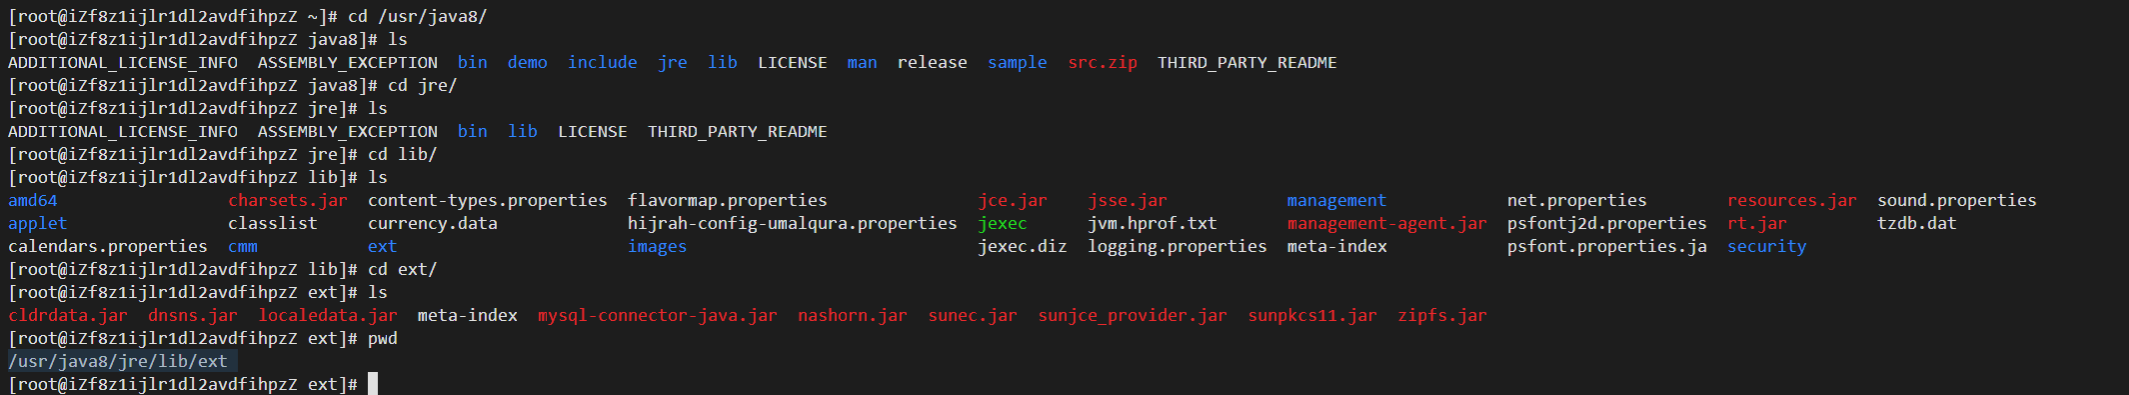
\includegraphics[width=15cm]{jdbc路径.png}
        \caption{/usr/java8/jre/lib/ext}
        \label{pic6}
    \end{figure}

    \item 实现平面文件.json存储到mysql
    \begin{lstlisting}
1.创建json数据
cd ~/file
vim data.json

#数据如下
[
    {
        "name": "张三",
        "age": 23,
        "gender": 1
    },{
        "name": "李四",
        "age": 24,
        "gender": 1
    },{
        "name": "小红",
        "age": 18,
        "gender": 0
    }
]
    \end{lstlisting}
    \begin{figure}[htp]
        \centering
        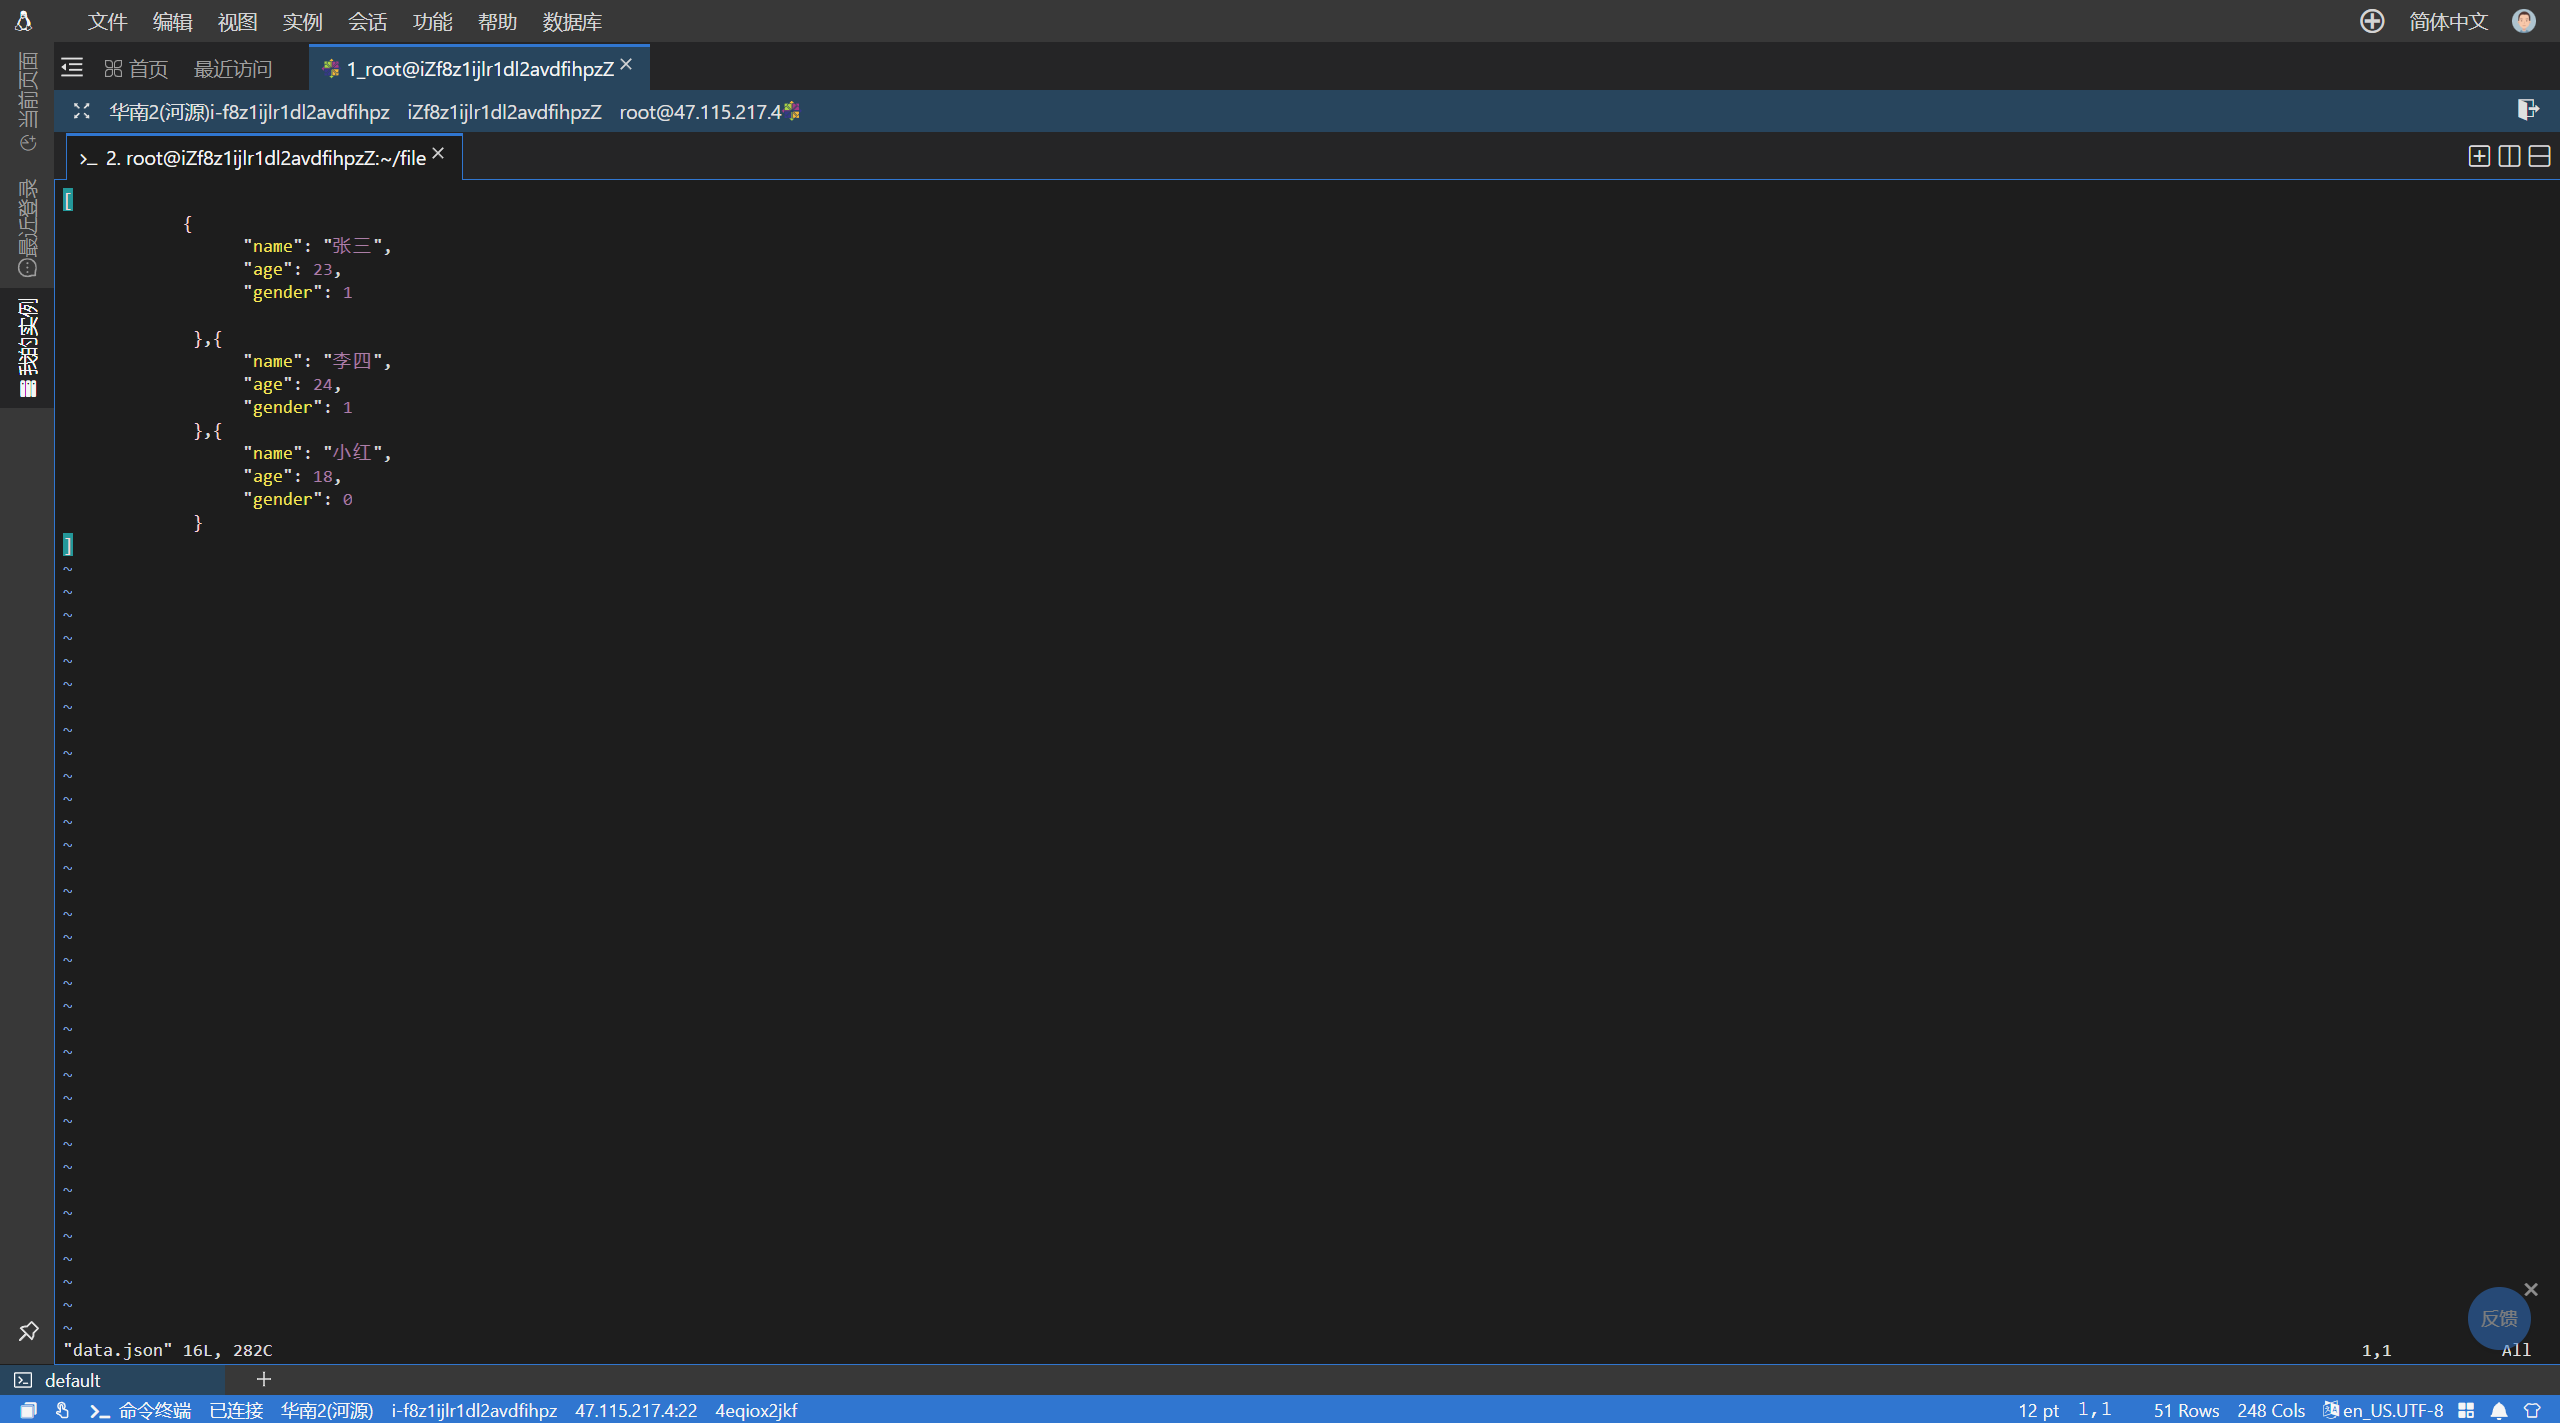
\includegraphics[width=15cm]{data.json.png}
        \caption{data.json}
        \label{pic6}
    \end{figure}
    \begin{lstlisting}
2.在数据库中创建表

CREATE TABLE `sys_user` (
  `id` bigint NOT NULL AUTO_INCREMENT COMMENT '用户ID',
  `name` varchar(50) NOT NULL DEFAULT '' COMMENT '姓名',
  `age`  int NOT NULL DEFAULT 0 COMMENT '年龄',
  `gender` tinyint NOT NULL COMMENT '性别,1:男,0:女',
  `create_time` timestamp NOT NULL DEFAULT CURRENT_TIMESTAMP COMMENT '创建时间',
  `is_deleted` tinyint NOT NULL DEFAULT '0' COMMENT '是否已删除',
  PRIMARY KEY (`id`) USING BTREE
) ENGINE=InnoDB DEFAULT  CHARSET=utf8mb4 COLLATE=utf8mb4_0900_ai_ci ROW_FORMAT=DYNAMIC COMMENT='用户表';

3.创建文件流

添加处理器:GetFile
点击工具栏的Processor,拖拽到画布中
    \end{lstlisting}
    \begin{figure}[htp]
        \centering
        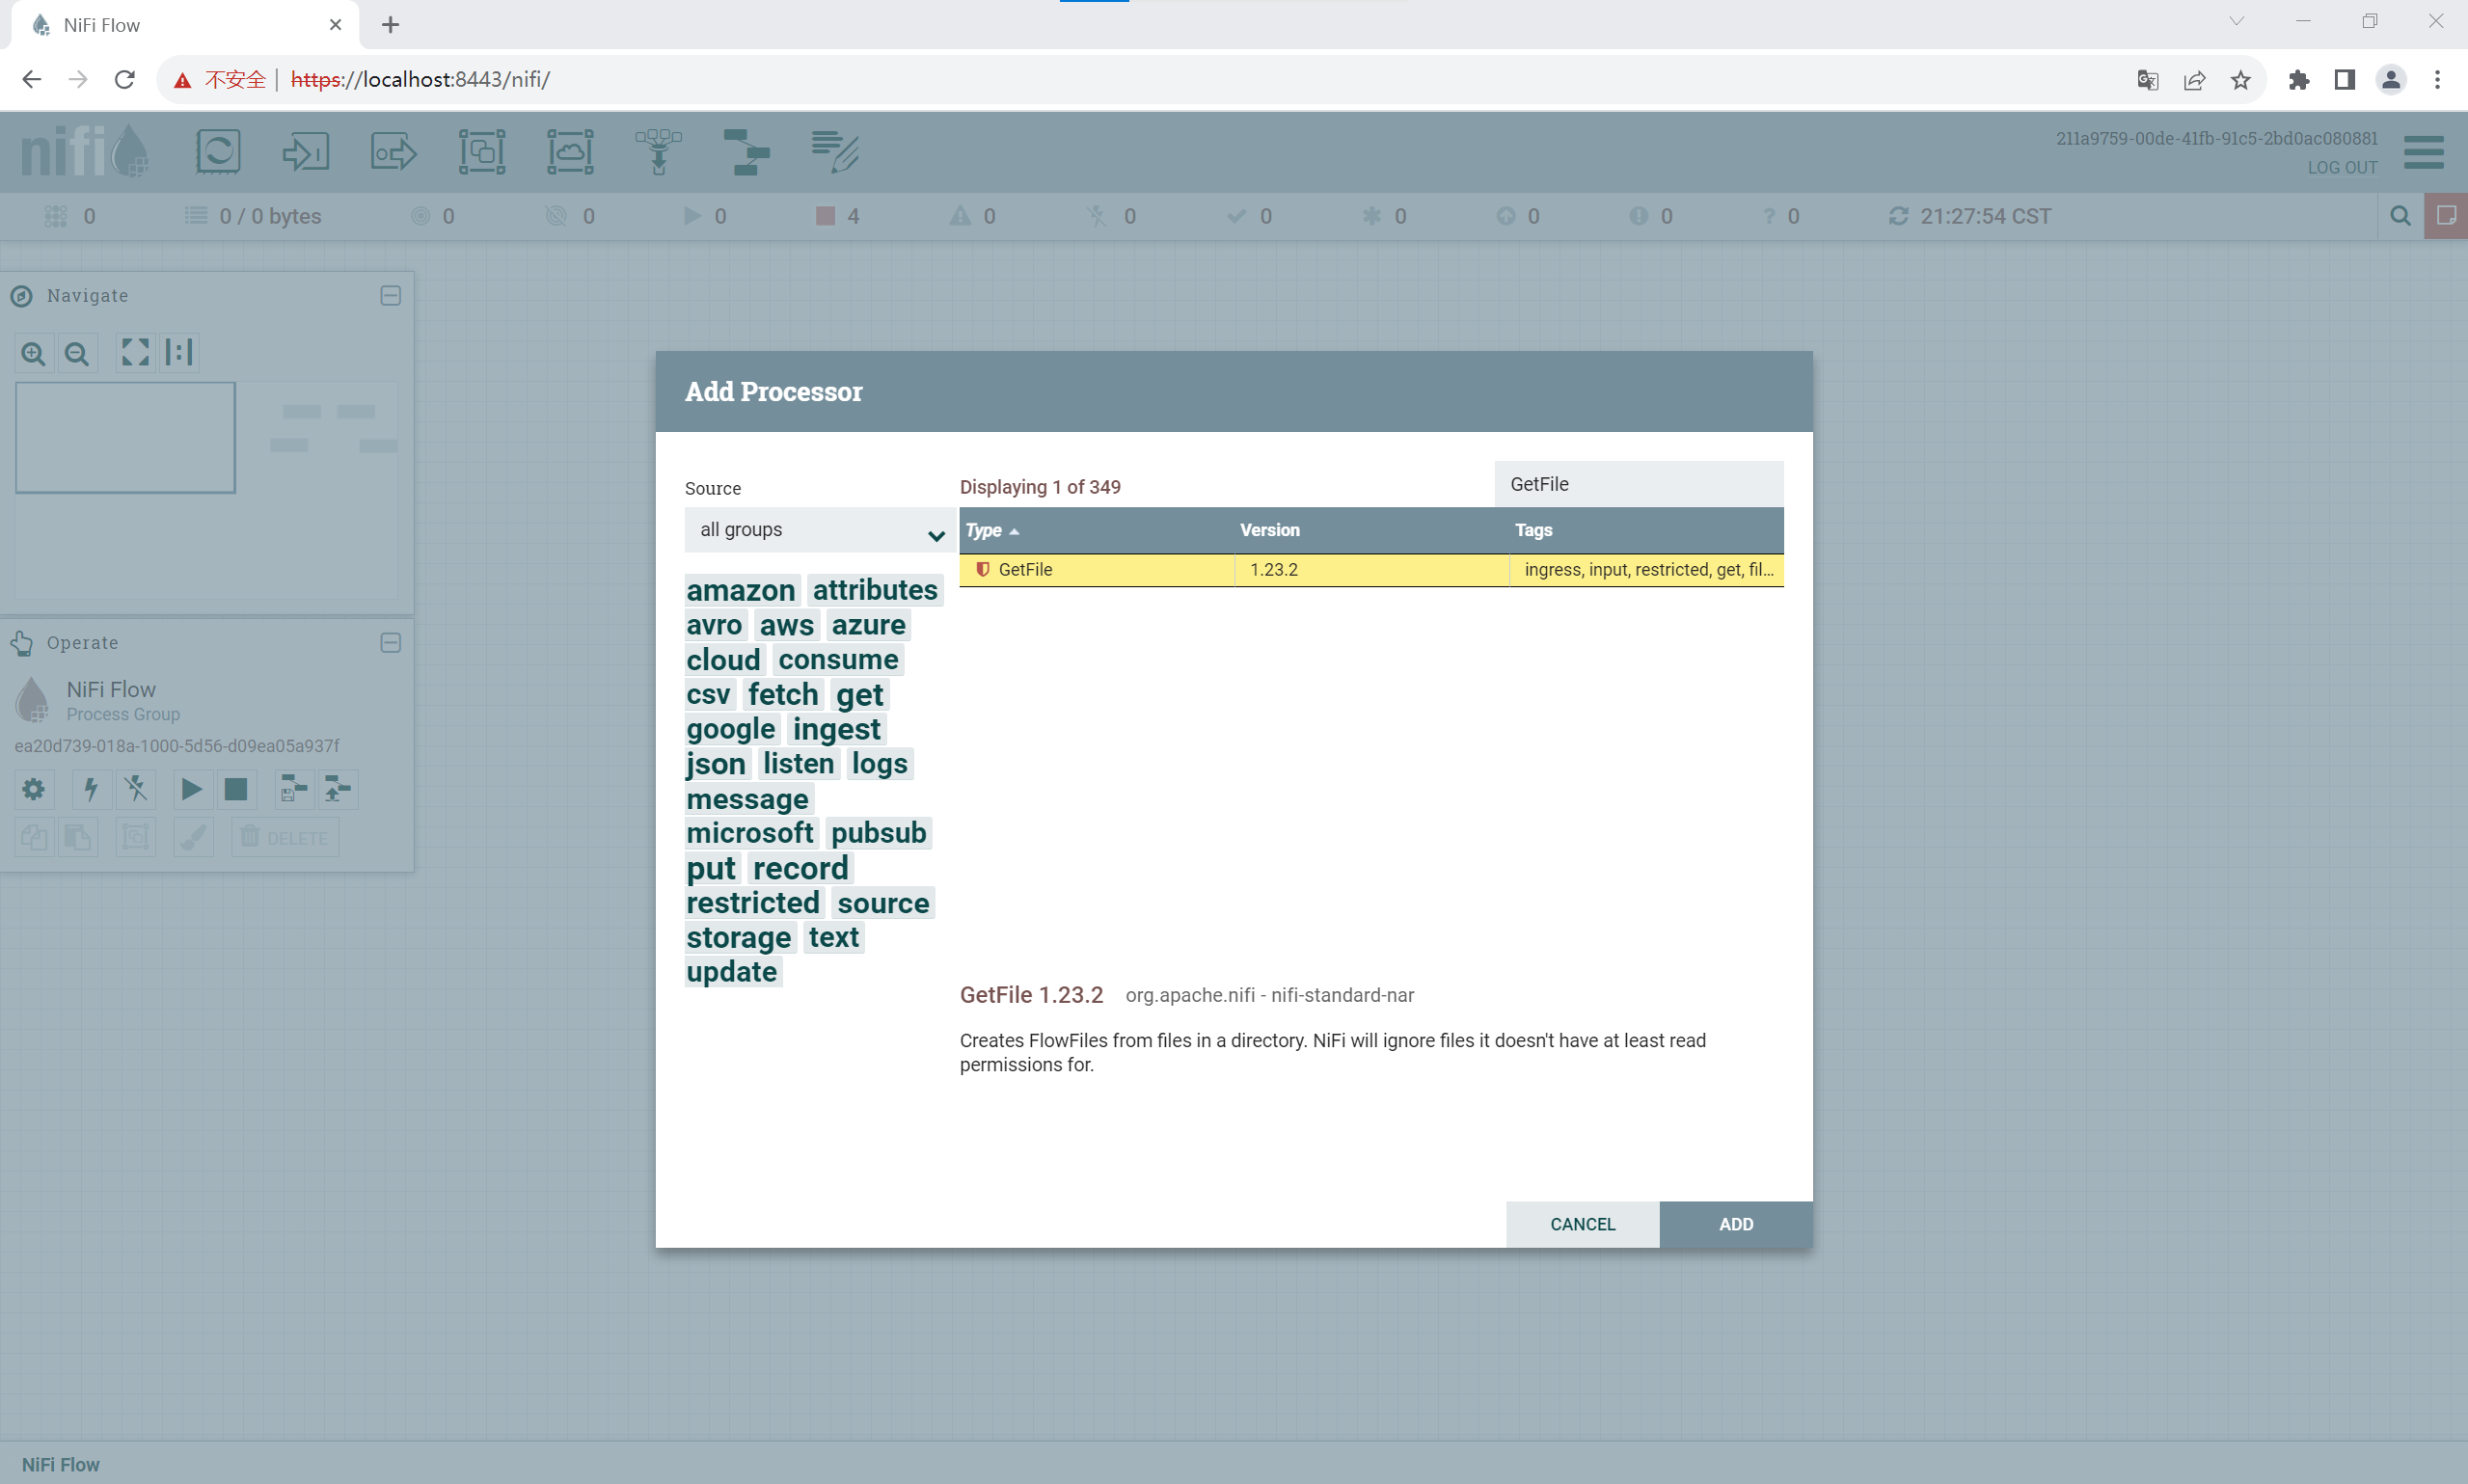
\includegraphics[width=13cm]{getFile.png}
        \caption{筛选GetFile,点击ADD添加到画布中}
        \label{}
    \end{figure}
    \begin{figure}[htp]
        \centering
        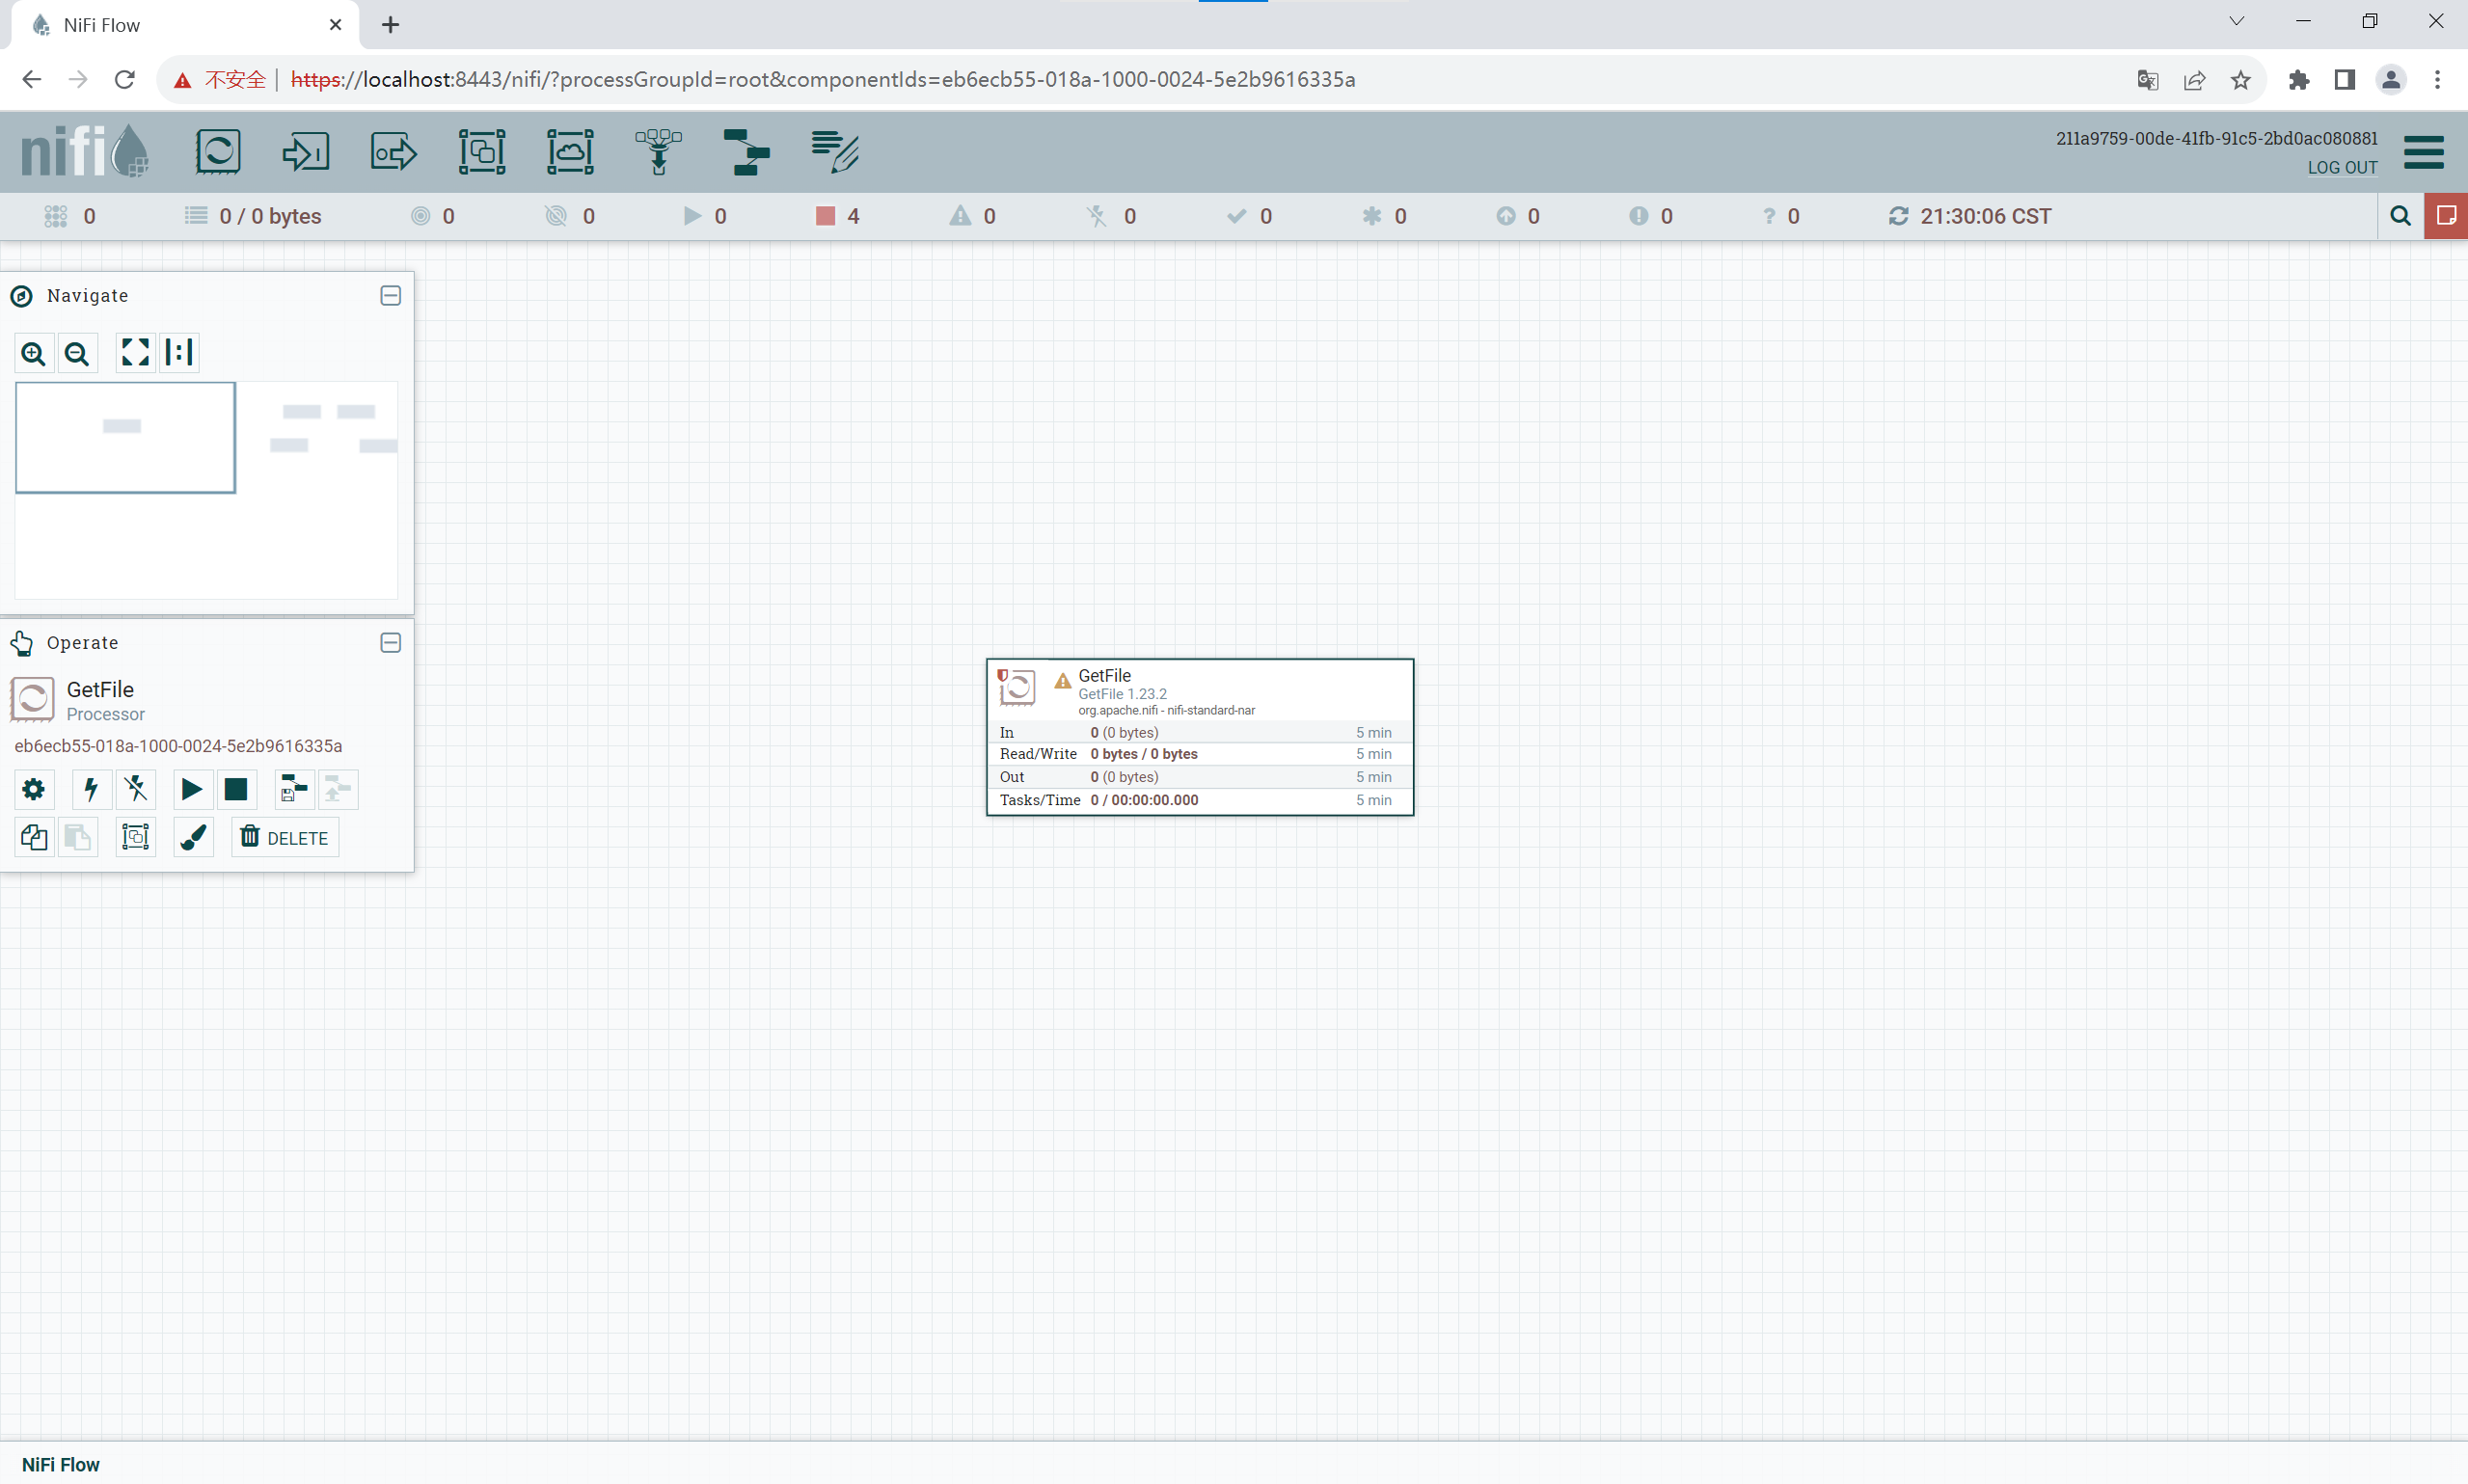
\includegraphics[width=13cm]{createGetFile.png}
        \caption{GetFile}
        \label{pic6}
    \end{figure}
    \begin{lstlisting}
配置GetFile处理器
双击添加的处理器,弹出对应的配置界面
    \end{lstlisting}
    \begin{figure}[htp]
        \centering
        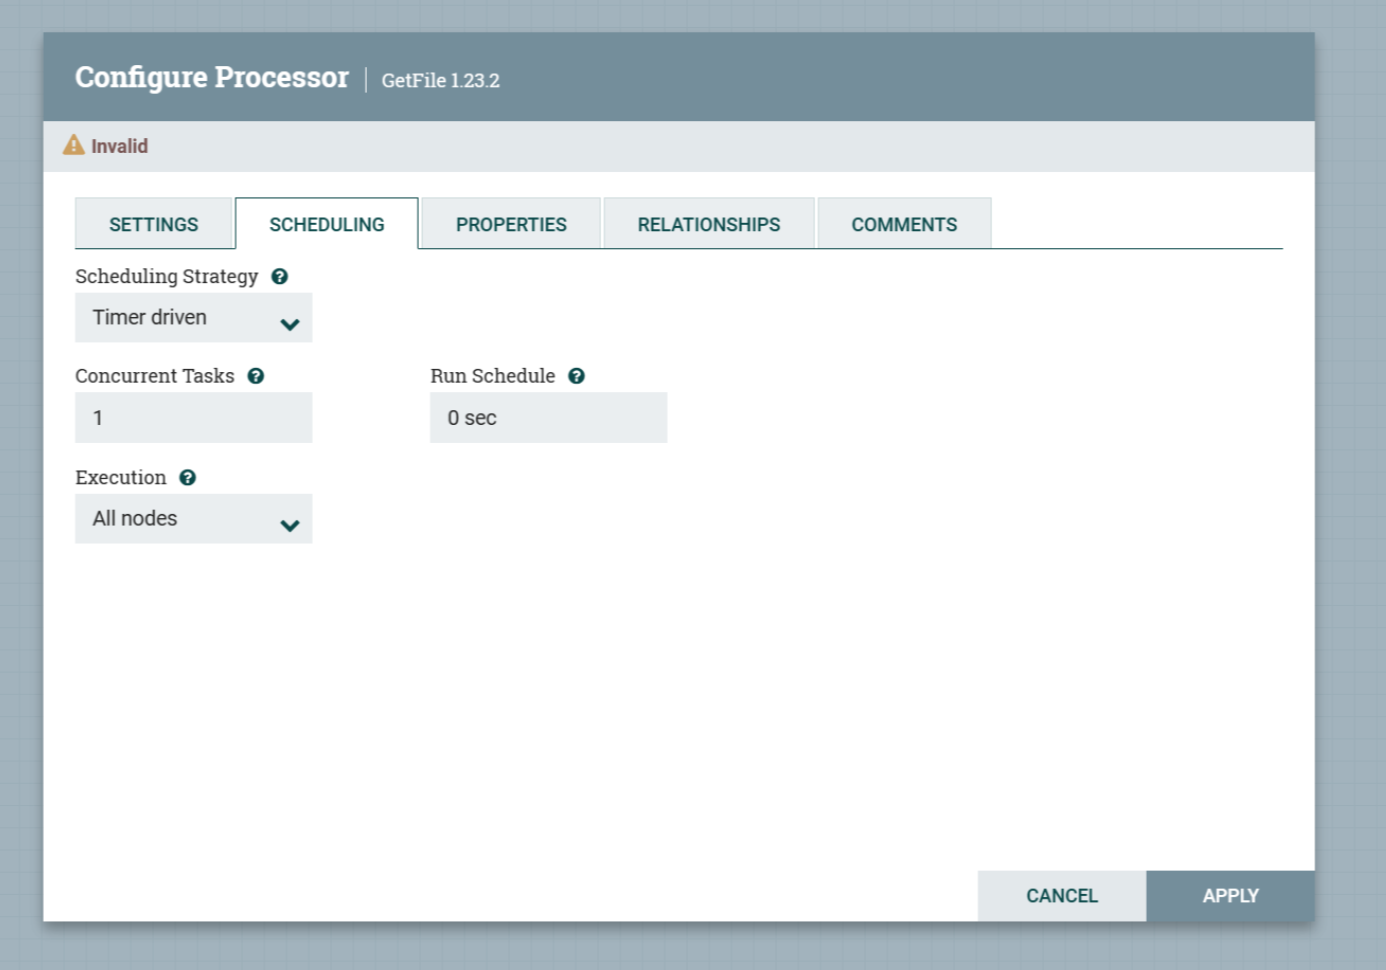
\includegraphics[width=13cm]{getfile配置界面.png}
        \caption{配置界面}
        \label{pic6}
    \end{figure}
    \begin{figure}[htp]
        \centering
        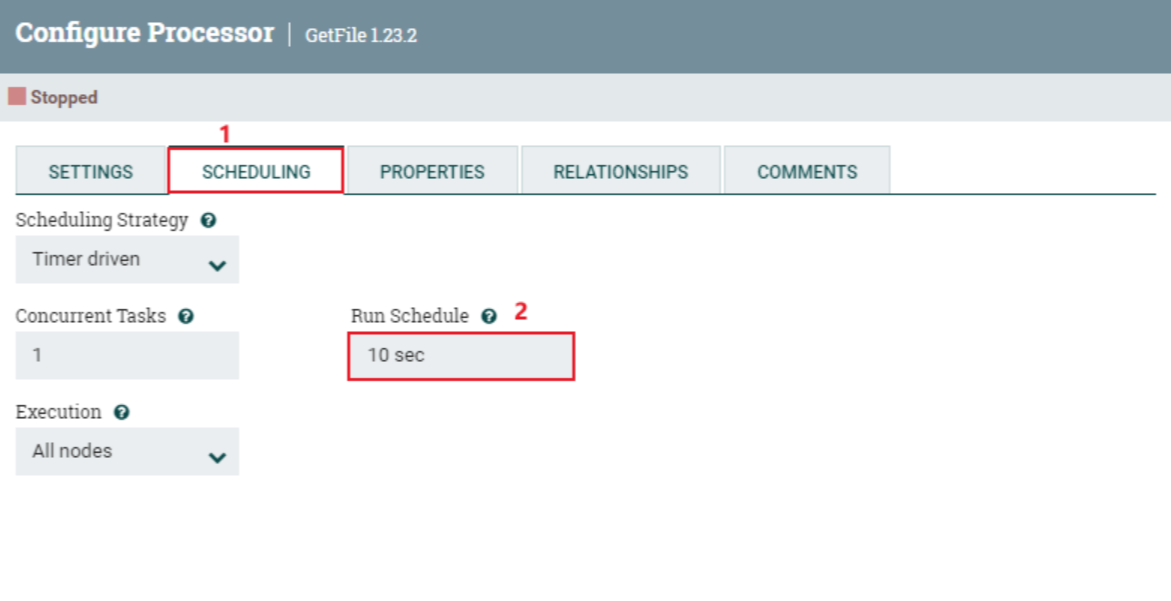
\includegraphics[width=13cm]{定时器10s.png}
        \caption{设置10s定时器}
        \label{pic6}
    \end{figure}
    \begin{figure}[htp]
        \centering
        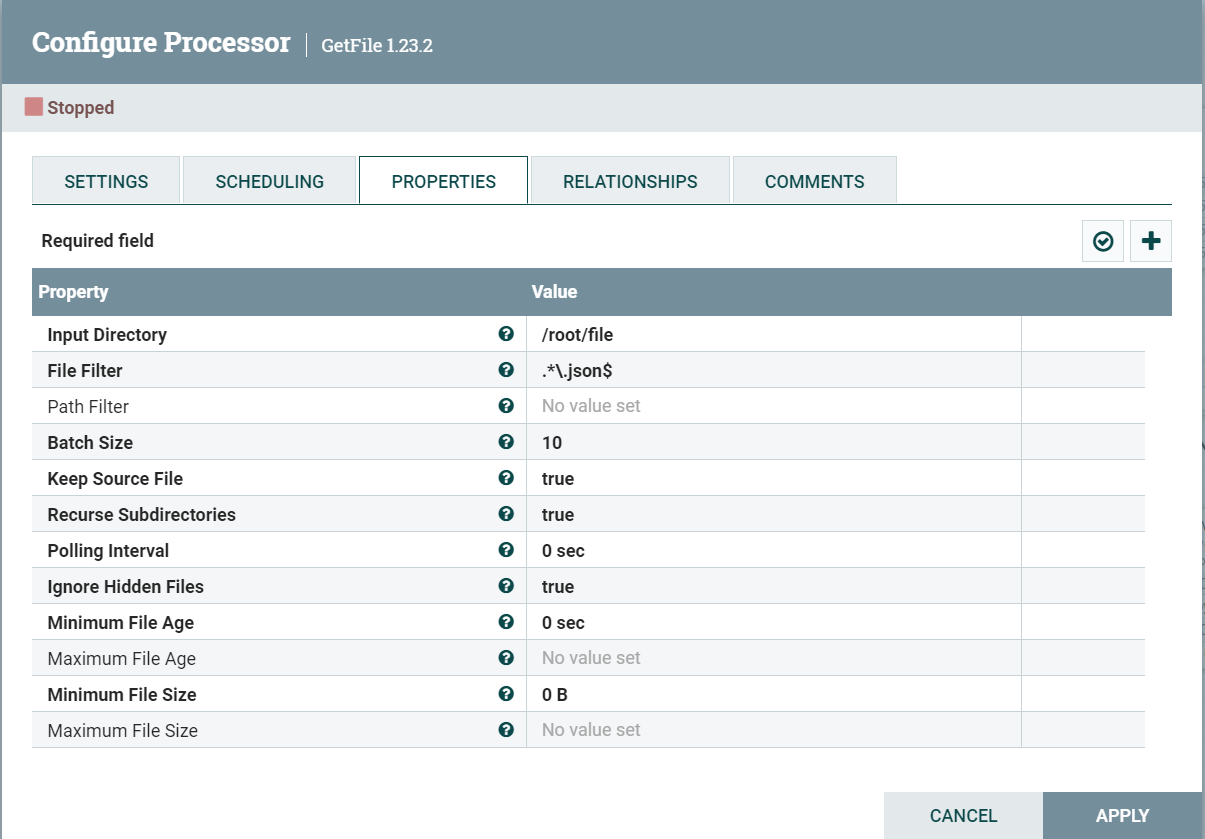
\includegraphics[width=13cm]{getfile配置2.png}
        \caption{设置文件路径}
        \label{pic6}
    \end{figure}
    \newpage
    \begin{lstlisting}
添加和配置处理器:SplitJson
    \end{lstlisting}
    \begin{figure}[htp]
        \centering
        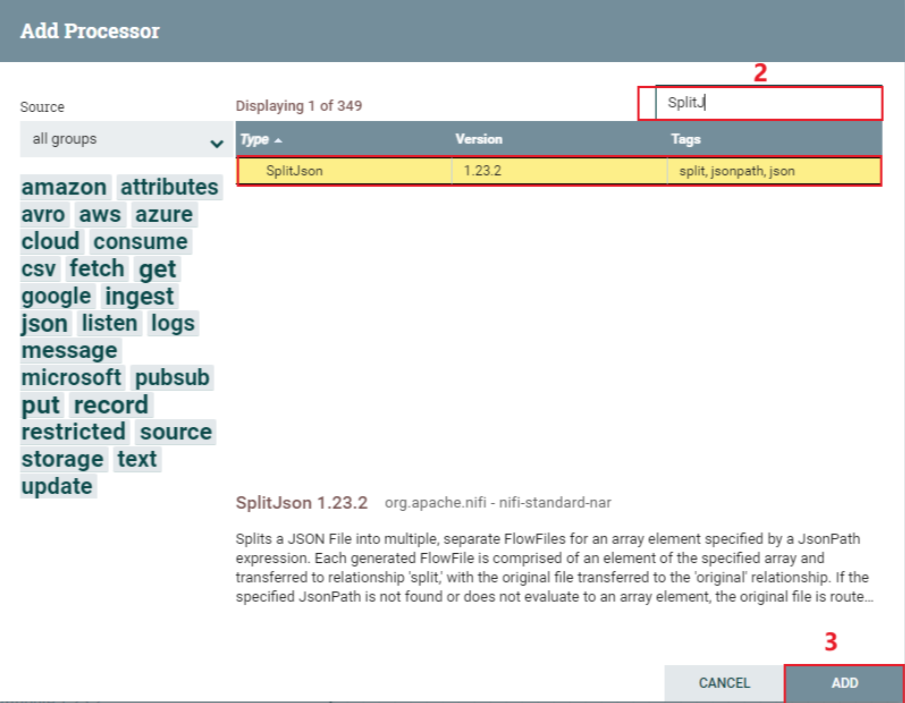
\includegraphics[width=13cm]{添加split.png}
        \caption{添加处理器SplitJson}
        \label{pic6}
    \end{figure}
    \begin{figure}[htp]
        \centering
        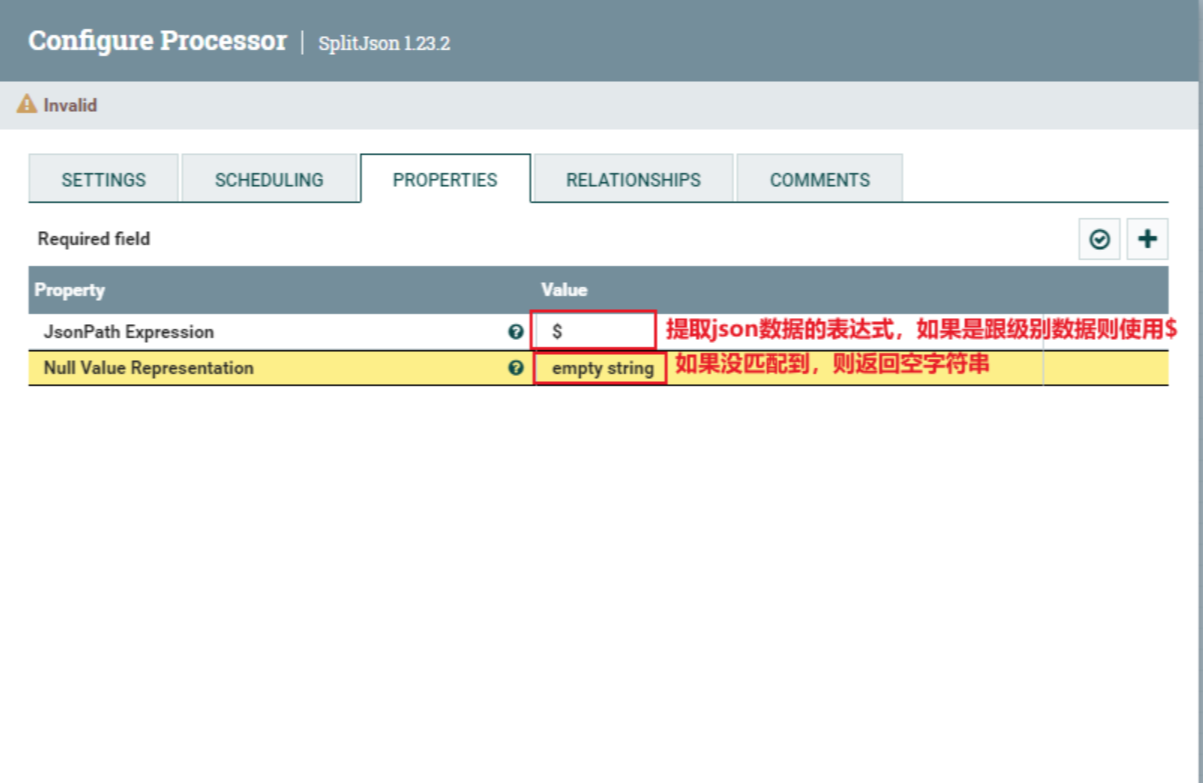
\includegraphics[width=13cm]{split配置.png}
        \caption{配置处理器SplitJson}
        \label{pic6}
    \end{figure}
    \newpage
    \begin{lstlisting}
连接处理器
将GetFile处理器和SplitJson处理器连接起来,勾选For Relationships,然后选择ADD
    \end{lstlisting}
    \begin{figure}[htp]
        \centering
        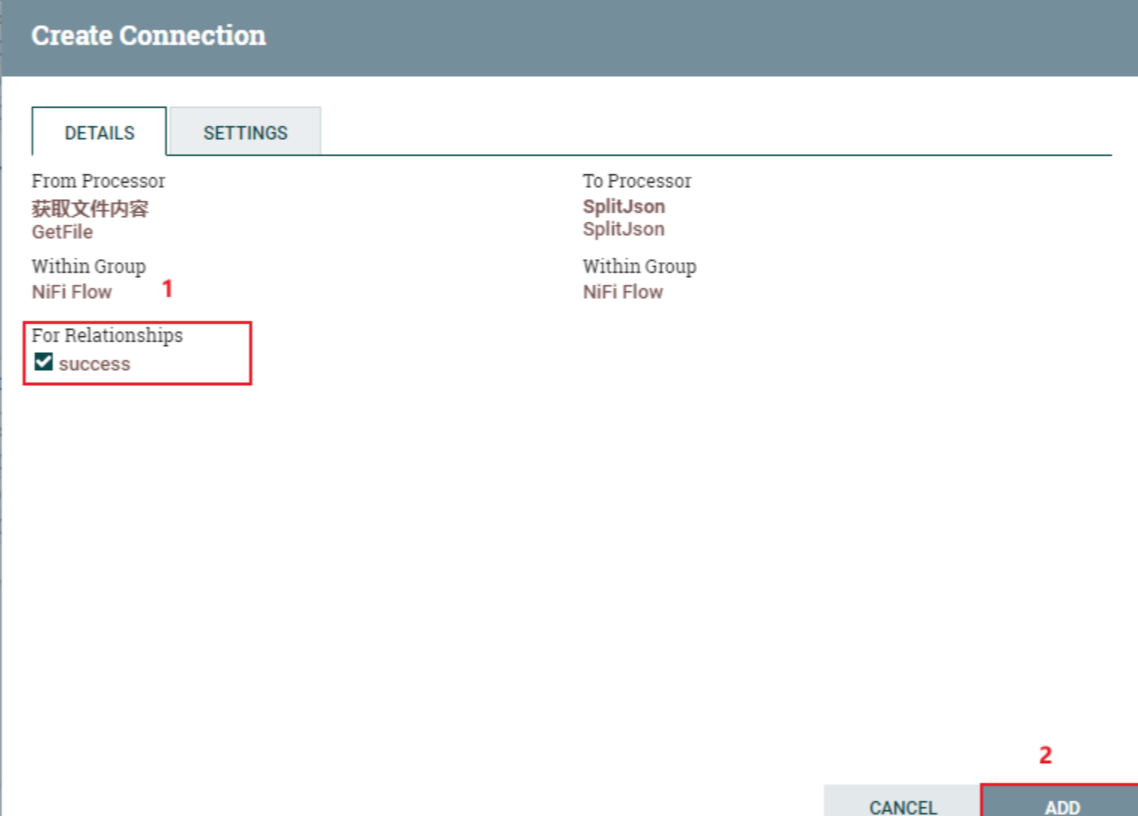
\includegraphics[width=13cm]{连接1.png}
        \caption{将GetFile处理器和SplitJson处理器连接}
        \label{pic6}
    \end{figure}
    \newpage
    \begin{lstlisting}
Json转为SQL
    \end{lstlisting}
    \begin{figure}[htp]
        \centering
        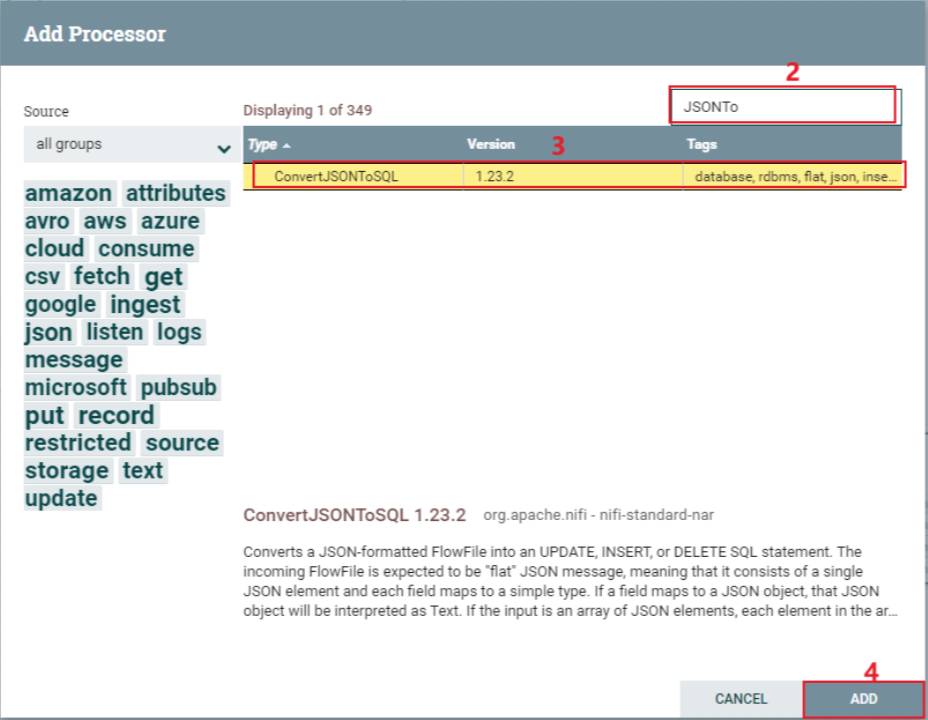
\includegraphics[width=13cm]{添加jsonTo.png}
        \caption{添加处理器ConvertJSONToSQL}
        \label{pic6}
    \end{figure}
    \begin{figure}[htp]
        \centering
        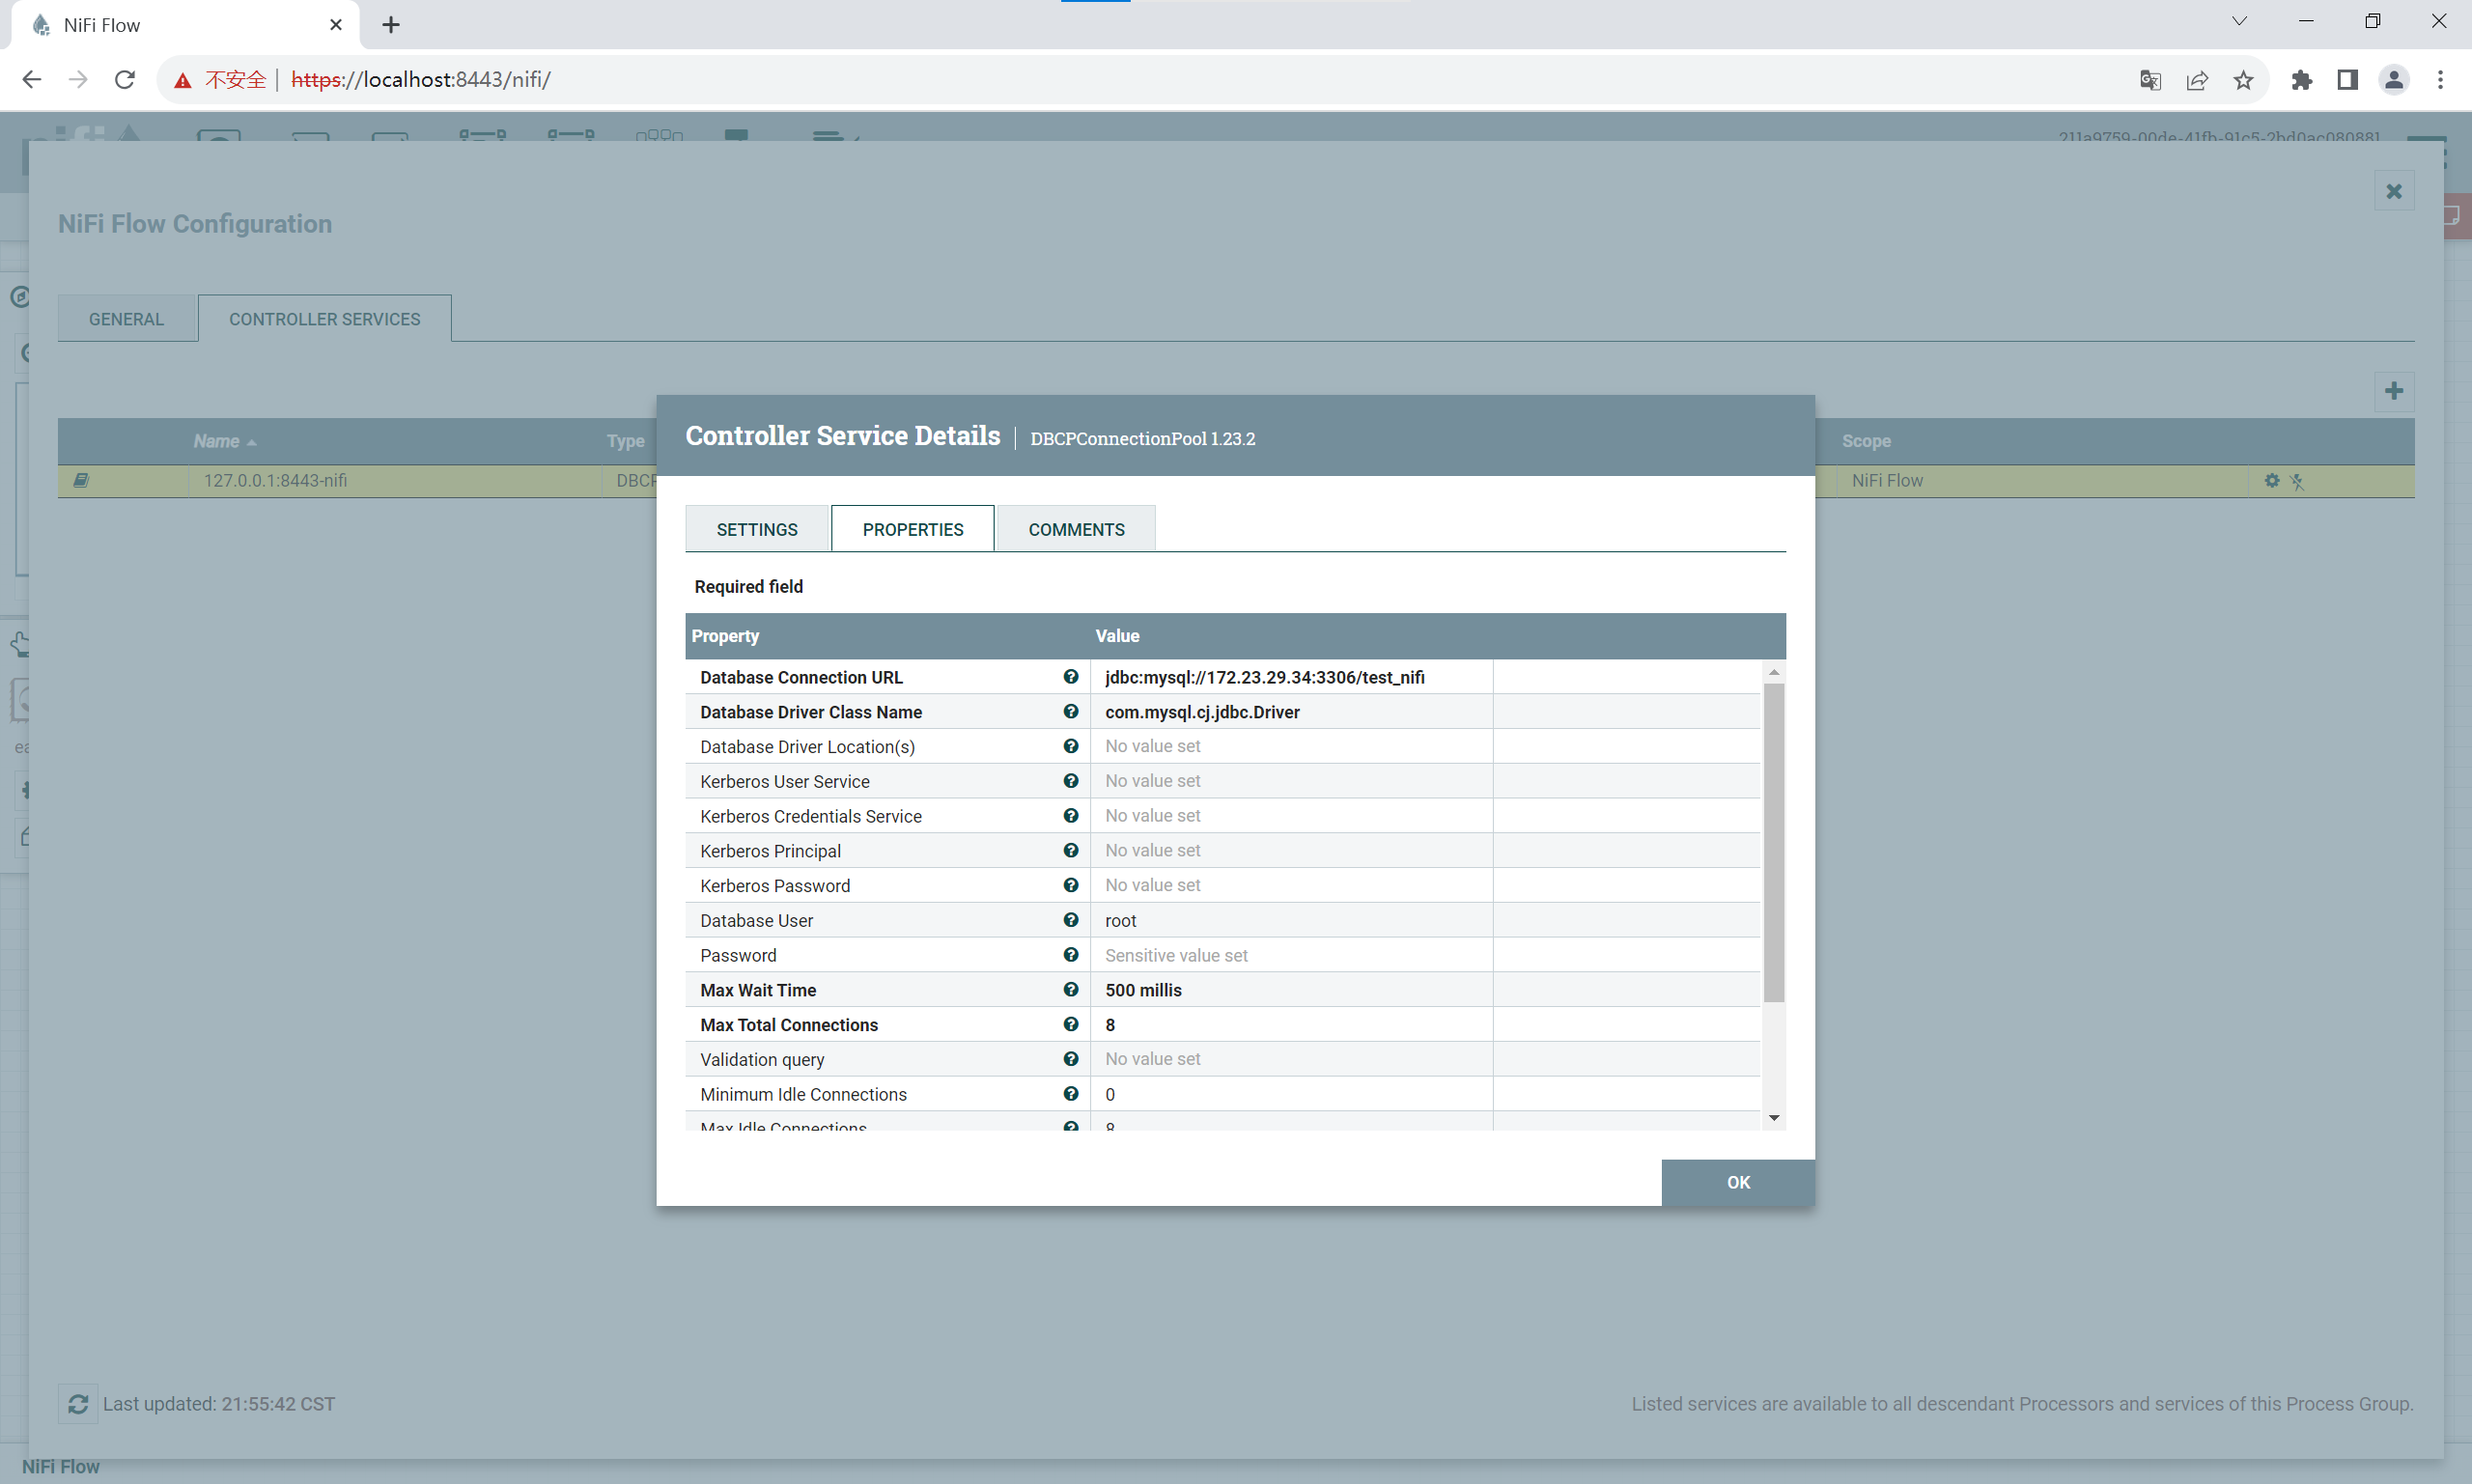
\includegraphics[width=13cm]{配置jsonTo.png}
        \caption{配置处理器ConvertJSONToSQL}
        \label{pic6}
    \end{figure}
    \begin{figure}[htp]
        \centering
        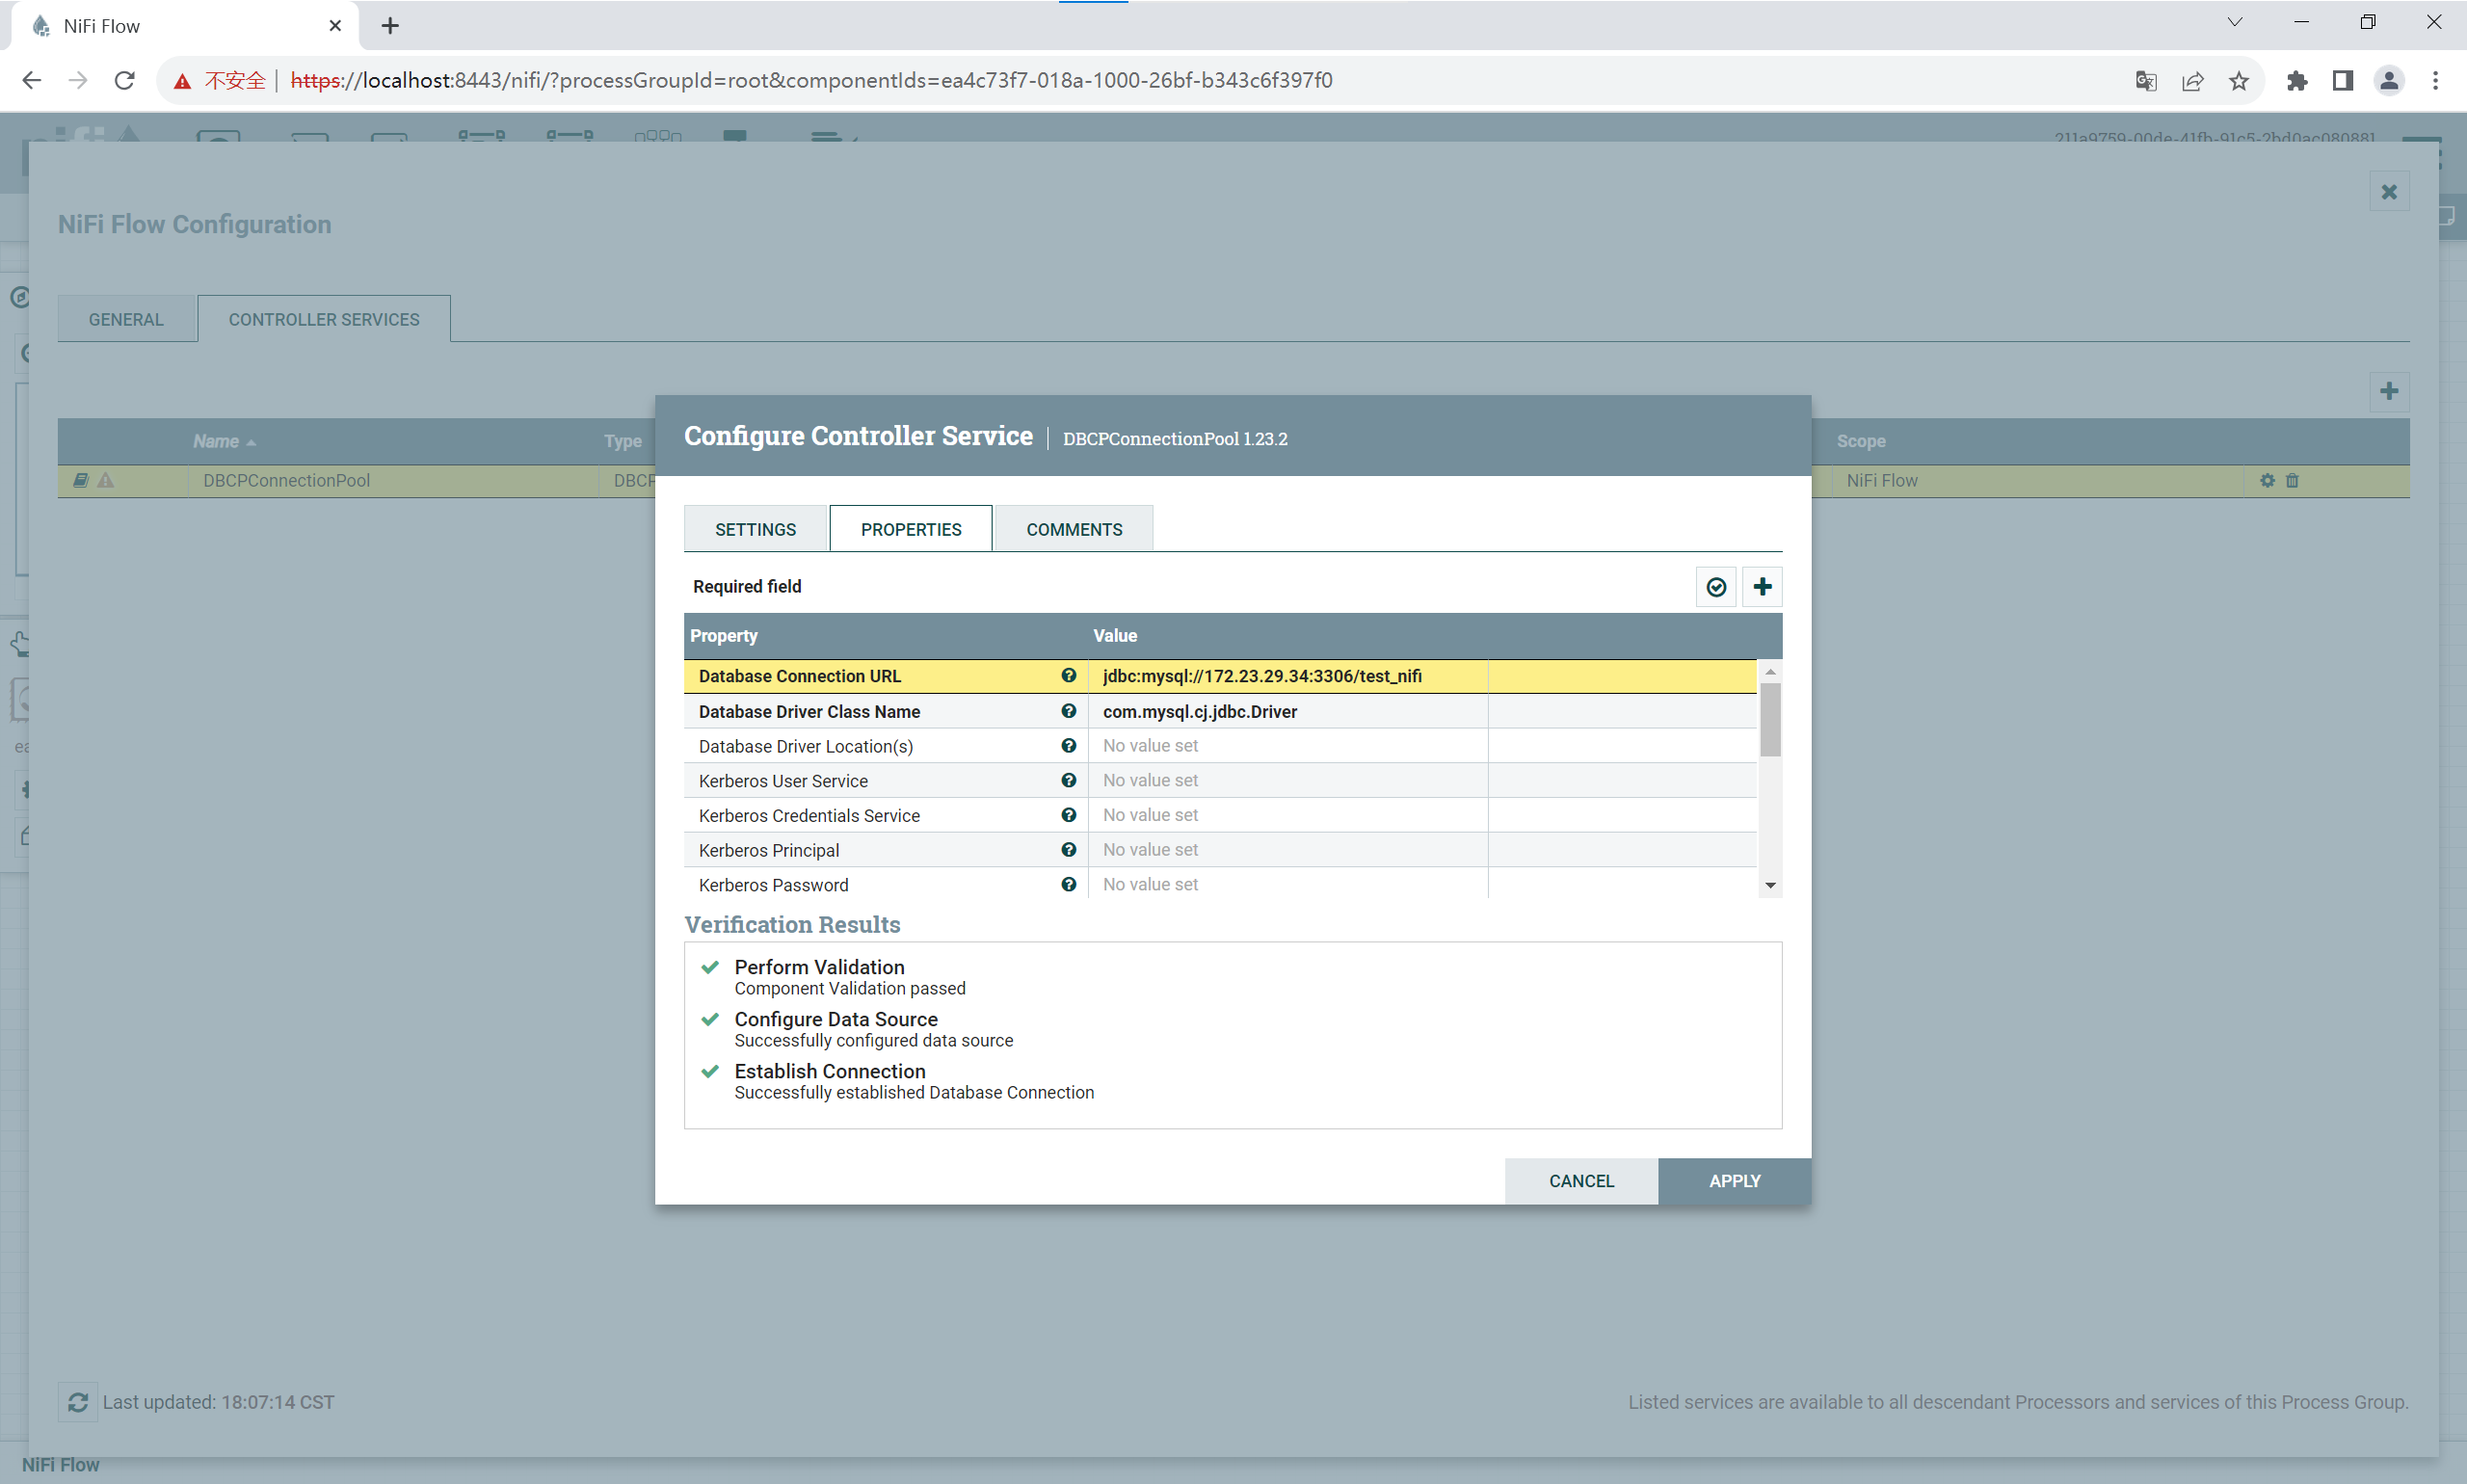
\includegraphics[width=13cm]{jdbc.png}
        \caption{测试jdbc连接}
        \label{pic6}
    \end{figure}
    \begin{figure}[htp]
        \centering
        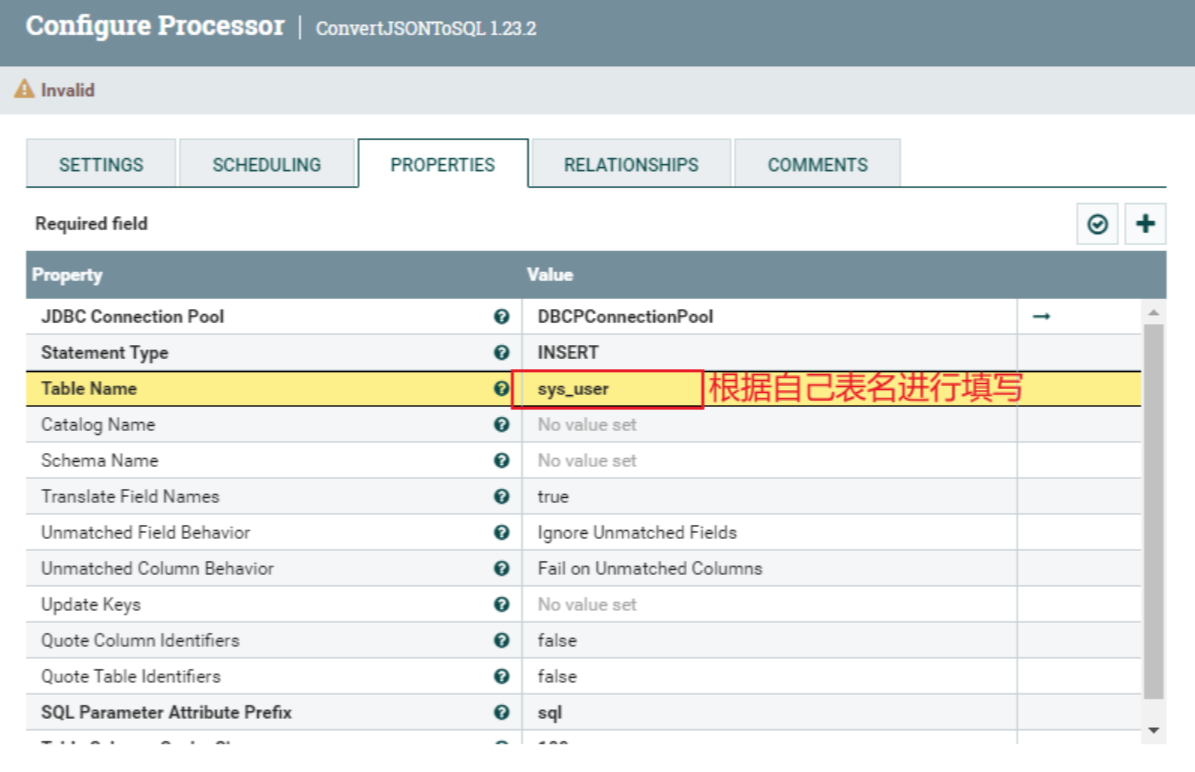
\includegraphics[width=13cm]{配置jsonTo2.png}
        \caption{配置Table Name和Statement Type}
        \label{pic6}
    \end{figure}
    \newpage
    \begin{lstlisting}
连接处理器
将SplitJson处理器和ConvertJSONToSQL处理器进行连接,Relationships选择split
    \end{lstlisting}
    \begin{figure}[htp]
        \centering
        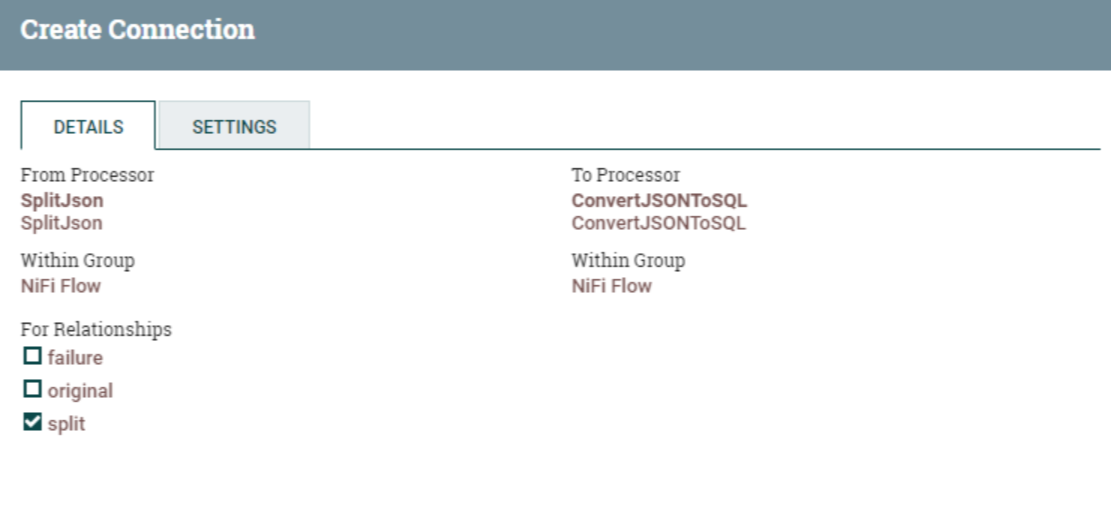
\includegraphics[width=13cm]{连接2.png}
        \caption{Relationships选择split}
        \label{pic6}
    \end{figure}
    \newpage
    \begin{lstlisting}
执行生成的SQL
添加处理器:PutSQL
    \end{lstlisting}
    \begin{figure}[htp]
        \centering
        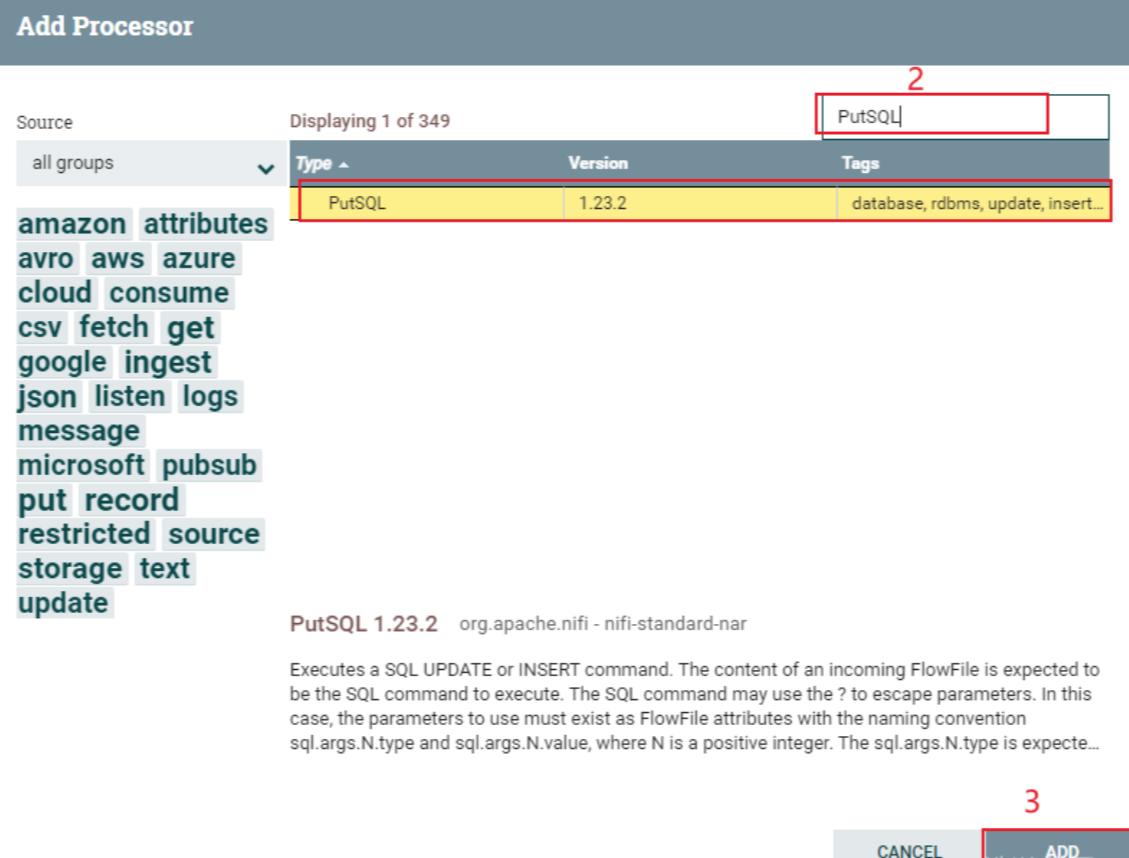
\includegraphics[width=13cm]{添加putsql.png}
        \caption{添加处理器:PutSQL}
        \label{pic6}
    \end{figure}
    \begin{figure}[htp]
        \centering
        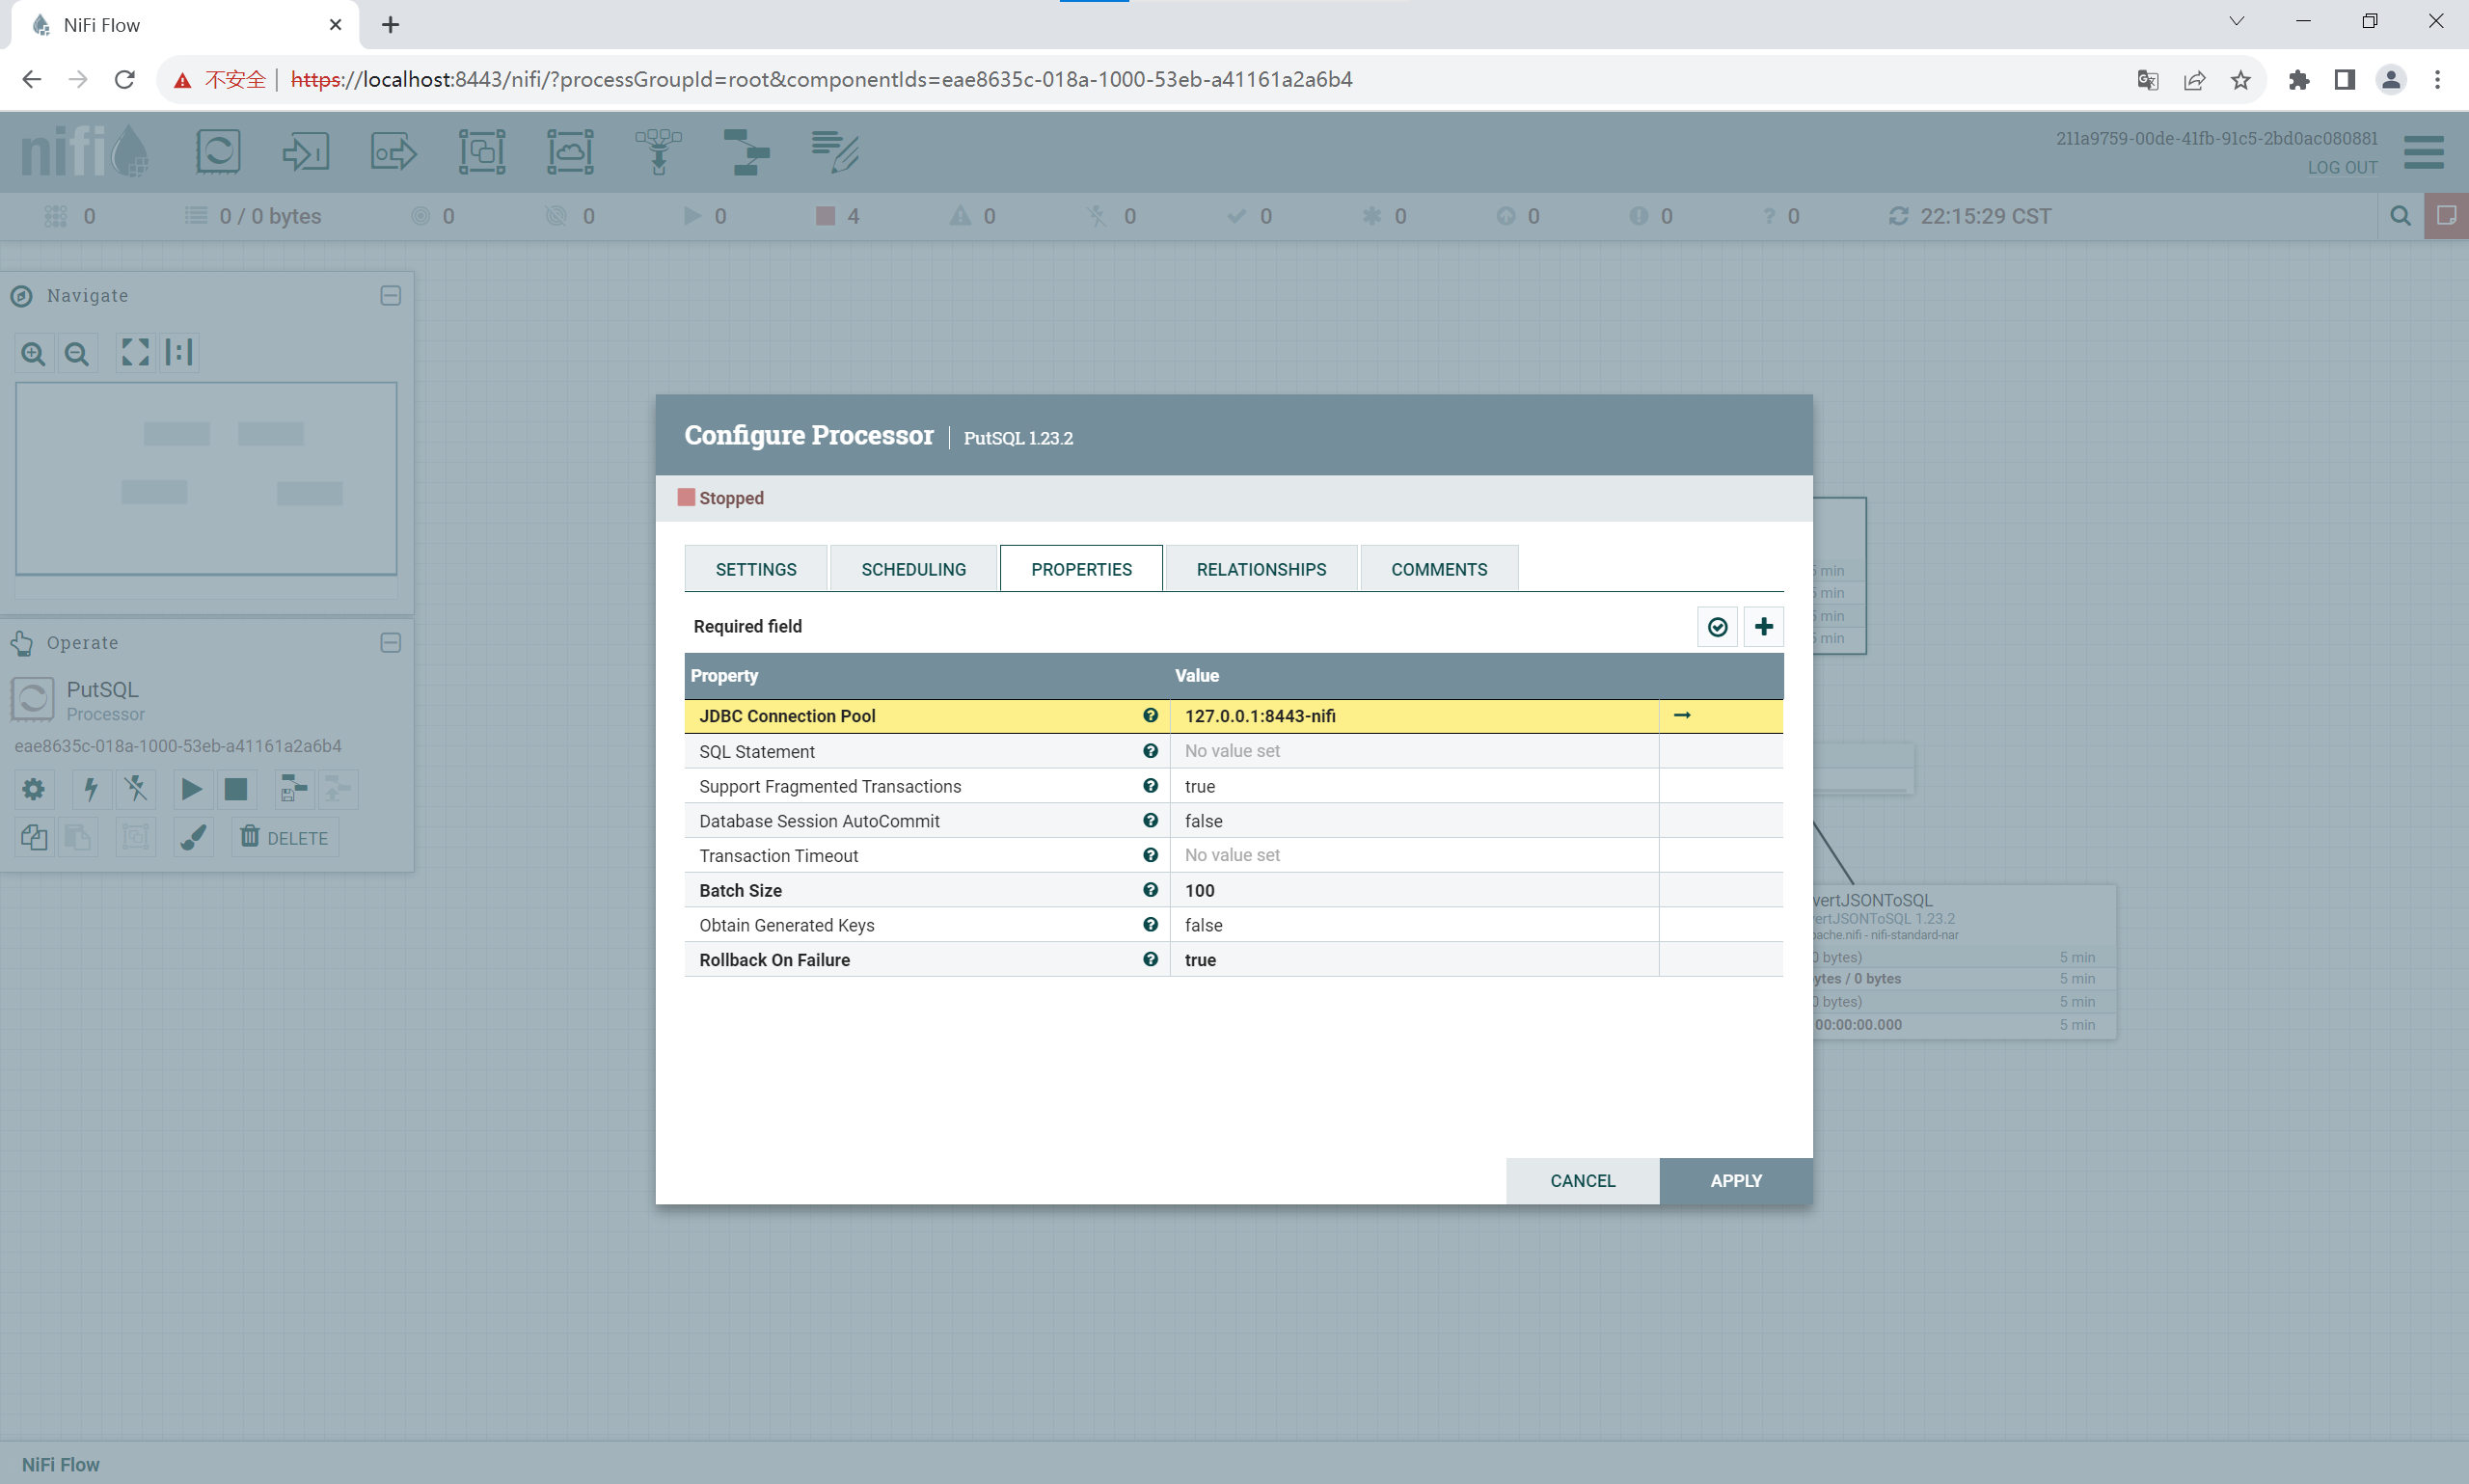
\includegraphics[width=13cm]{配置putsql.png}
        \caption{配置putsql}
        \label{pic6}
    \end{figure}
    \newpage
    \begin{lstlisting}
连接处理器
将ConvertJSONToSQL处理器和PutSQL处理器进行连接,Relationships选择sql
    \end{lstlisting}
    \begin{figure}[htp]
        \centering
        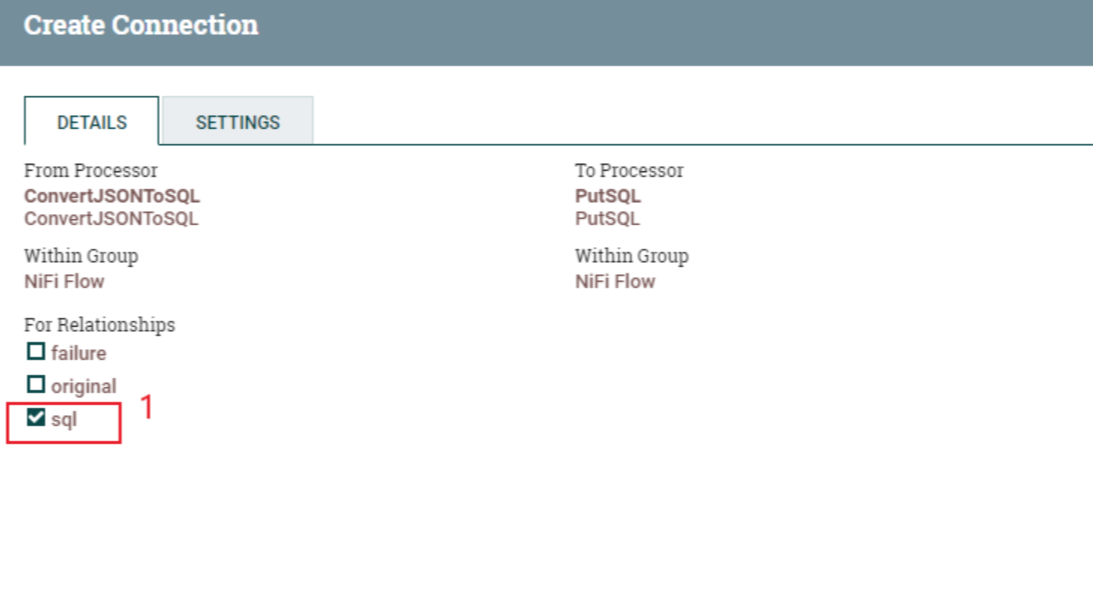
\includegraphics[width=13cm]{连接3.png}
        \caption{Relationships选择sql}
        \label{pic6}
    \end{figure}
    \newpage
    
    \item 实验结果
    \begin{figure}[htp]
        \centering
        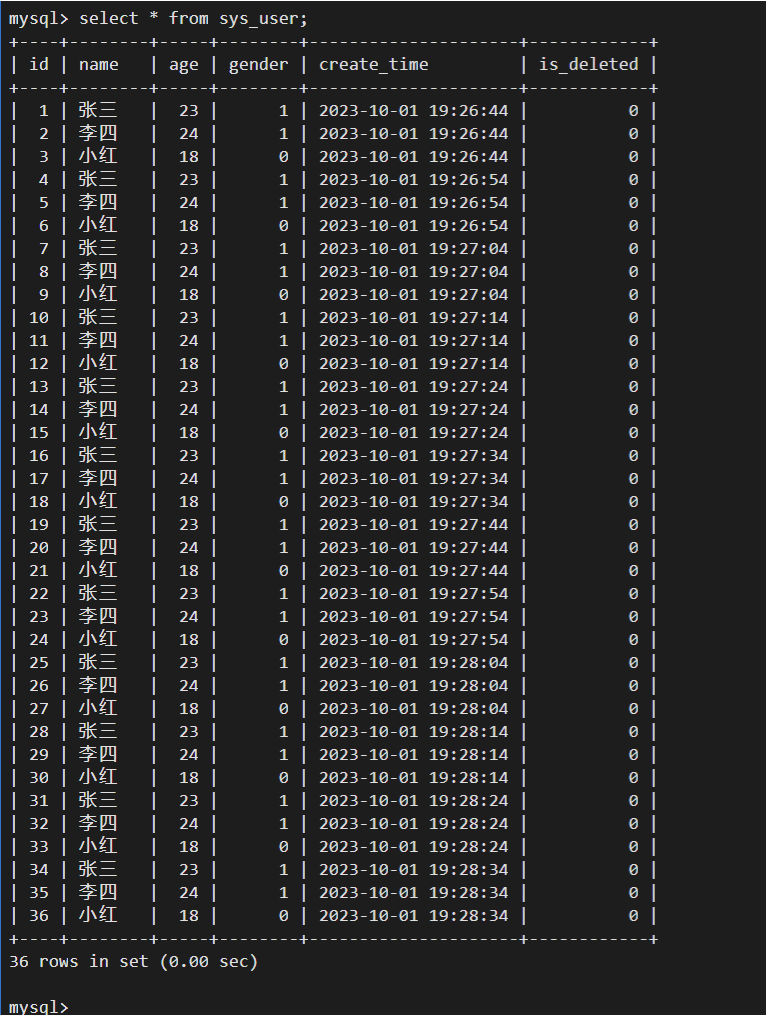
\includegraphics[width=13cm]{re_database.png}
        \caption{sql数据库中的sys-user}
        \label{pic6}
    \end{figure}
    \begin{lstlisting}
可以很清晰的看到当运行这个数据流时,数据库的记录每10秒添加一次记录,
这些添加的内容恰好就是data.json的内容。
    \end{lstlisting}
    \begin{figure}[htp]
        \centering
        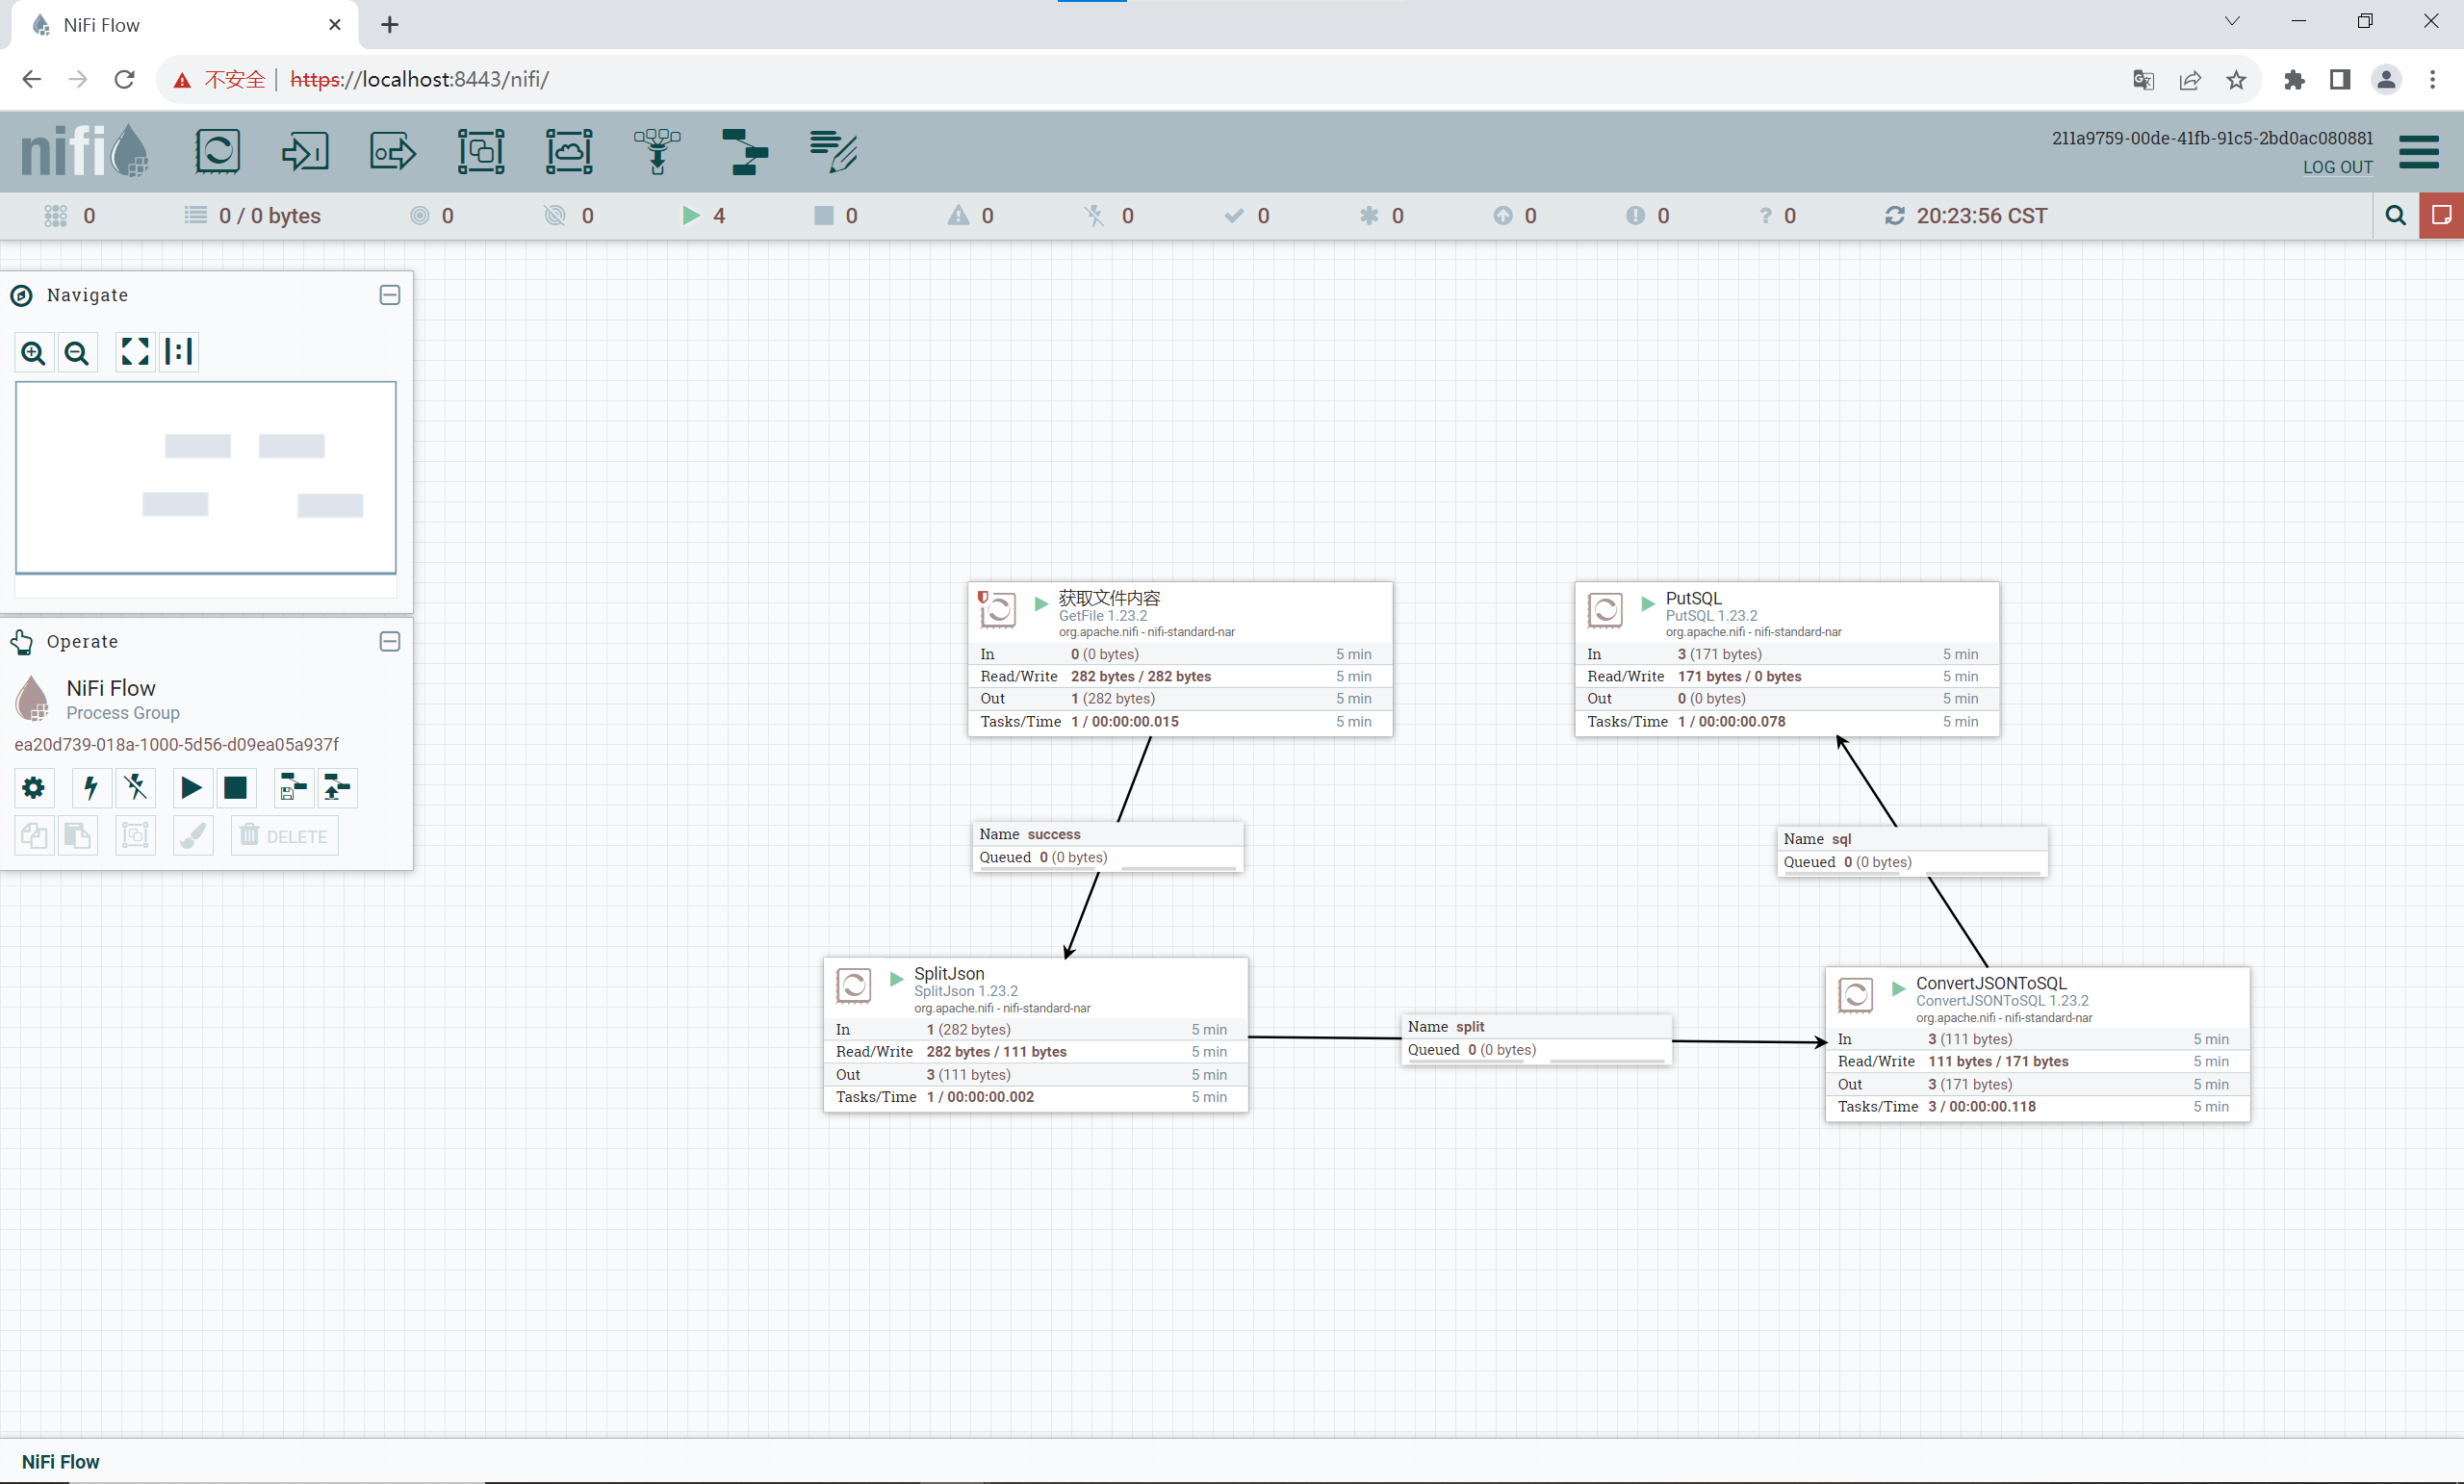
\includegraphics[width=13cm]{re_web_nifi.png}
        \caption{最终配置结果}
        \label{pic6}
    \end{figure}
    \newpage
\end{enumerate}


\section{任务四 使用 Flume 收集日志}

\begin{enumerate}
    \item 安装和配置flume
    \begin{lstlisting}
1.使用wget命令 从清华源下载安装包
wget https://mirrors.tuna.tsinghua.edu.cn/apache/flume/1.11.0/apache-flume-1.11.0-bin.tar.gz

2.解压安装包到 /opt目录下
tar -zxf apache-flume-1.11.0-bin.tar.gz -C /opt/

3.重命名flume
mv apache-flume-1.11.0-bin flume

4.进入/opt/flume/conf目录
cd /opt/flume/conf

5先复制一份flume-env.sh.template文件
cp flume-env.sh.template flume-env.sh

6修改flume-env.sh的Java_home
vim flume-env.sh
export JAVA_HOME=/usr/java8
    \end{lstlisting}
    \begin{figure}[htp]
        \centering
        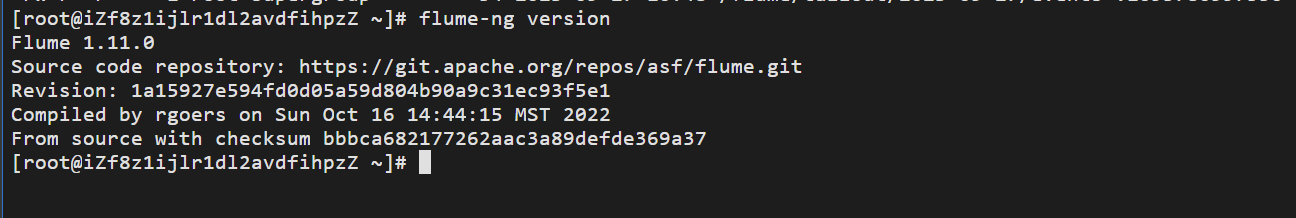
\includegraphics[width=15cm]{flume_version.png}
        \caption{验证flume安装成功}
        \label{pic7}
    \end{figure}
    \item 配置 Flume 以收集日志并将其存储在 HDFS 中
    \begin{lstlisting}
flume 提供了 Taildir Source,可实时监控一批文件,并记录每个文件最新消费位置,agent进程重启后不会有重复消费的问题。
Flume核心配置
tailDirSource配置

a1.sources = r1
a1.sources.r1.type = TAILDIR
a1.sources.r1.channels = c1
a1.sources.r1.positionFile = /export/servers/flume/taildir_position.json
a1.sources.r1.filegroups = f1 f2
a1.sources.r1.filegroups.f1 = /export/data/test1/example.log
a1.sources.r1.filegroups.f2 = /export/data/test2/.*log.*

##配置说明

filegroups

指定filegroups,可以有多个,以空格分隔;(TailSource可以同时监控tail多个目录中的文件)
positionFile

配置检查点文件的路径,检查点文件会以json格式保存已经tail文件的位置,解决了断点不能续传的缺陷。
filegroups.

配置每个filegroup的文件绝对路径,文件名可以用正则表达式匹配
sink配置
本次将日志采集到HDFS中,需要使用HDFSSink文件。HDFSSink需要配置滚动属性。

基于hdfs文件副本数
配置项:hdfs.minBlockReplicas
默认值:和hdfs的副本数一致
说明
hdfs.minBlockReplicas是为了让flume感知不到hdfs的块复制,这样滚动方式配置(比如时间间隔、文件大小、events数量等)才不会受影响
示例说明:
假如hdfs的副本为3,配置的滚动时间为10秒,那么在第二秒的时候,flume检测到hdfs在复制块,这时候flume就会滚动,这样导致flume的滚动方式受到影响。所以通常hdfs.minBlockReplicas配置为1,就检测不到副本的复制了。但是hdfs的实际副本还是3

--------
完整版配置文件
vim /opt/flume/conf/log2hdfs.conf

# Name the components on this agent
a1.sources = r1
a1.sinks = k1
a1.channels = c1

a1.sources.r1.type = TAILDIR
a1.sources.r1.positionFile = /opt/flume/taildir_position.json
a1.sources.r1.filegroups = f1
a1.sources.r1.filegroups.f1 = /export/data/test1/example.log

# Describe the sink
#指定hdfs sink
a1.sinks.k1.type = hdfs
#hdfs目录,带有时间信息
a1.sinks.k1.hdfs.path = /flume/tailout/%Y-%m-%d/
#生成的hdfs文件名的前缀
a1.sinks.k1.hdfs.filePrefix = events-
#指定滚动时间,默认是30秒,设置为0表示禁用该策略
a1.sinks.k1.hdfs.rollInterval = 0
#指定滚动大小,设置为0表示禁用该策略
a1.sinks.k1.hdfs.rollSize = 200000000
#指定滚动条数
a1.sinks.k1.hdfs.rollCount = 0
a1.sinks.k1.hdfs.batchSize = 100
a1.sinks.k1.hdfs.useLocalTimeStamp = true
#副本策略
a1.sinks.k1.hdfs.minBlockReplicas=1
#生成的文件类型,默认是Sequencefile,可用DataStream,则为普通文本
a1.sinks.k1.hdfs.fileType = DataStream

# Use a channel which buffers events in memory
a1.channels.c1.type = memory
a1.channels.c1.capacity = 1000
a1.channels.c1.transactionCapacity = 100

# Bind the source and sink to the channel
a1.sources.r1.channels = c1
a1.sinks.k1.channel = c1

--------------
启动flume agent采集数据
创建目录
mkdir -p /opt/data/test1/

进入test1中创建log文件
touch example.log

flume启动命令
flume-ng agent --conf-file conf/log2hdfs.conf -name a1 -Dflume.root.logger=INFO,console
    \end{lstlisting}
    \newpage
    \begin{figure}[htp]
        \centering
        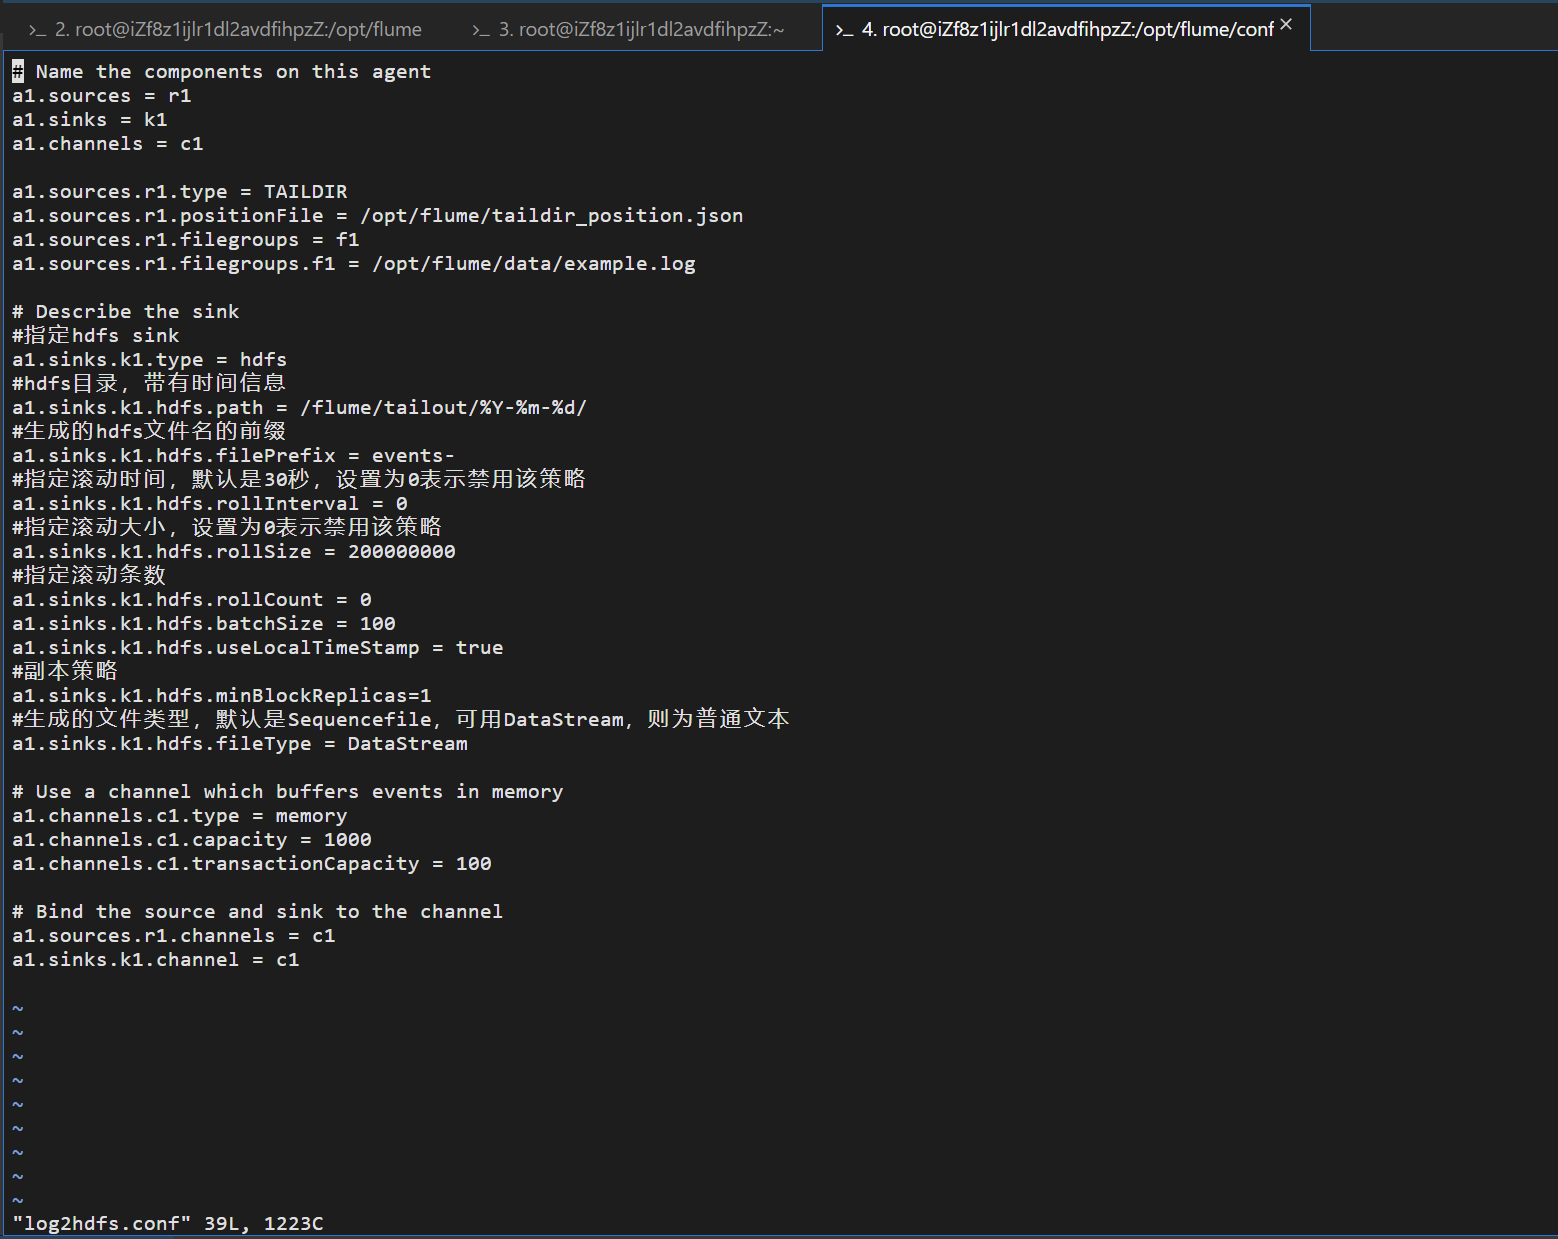
\includegraphics[width=15cm]{log2hdfs.conf.png}
        \caption{log2hdfs.conf的内容}
        \label{pic6}
    \end{figure}
    \begin{figure}[htp]
        \centering
        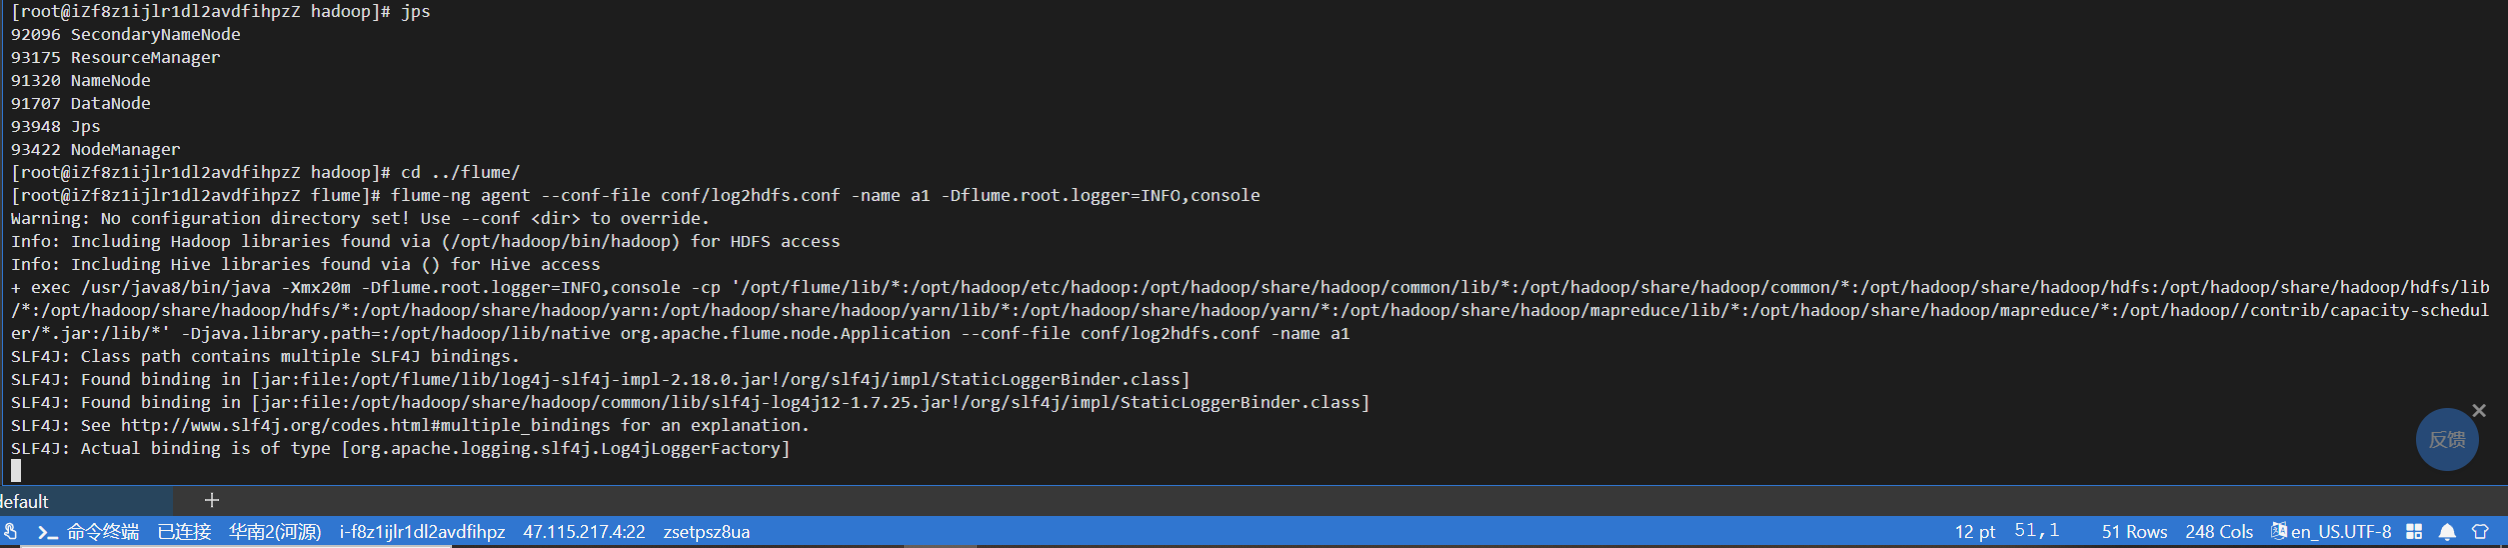
\includegraphics[width=15cm]{flume_monitor.png}
        \caption{flume flume-ng agent命令}
        \label{pic5}
    \end{figure}
    \newpage
    \begin{lstlisting}
1.新建一个master节点
打开一个新的命令行终端
cd /opt/flume/data/

重复输入以下命令
"hello BIG DATA" >> example.log
"hello world" >> example.log
    \end{lstlisting}
    \begin{figure}[htp]
        \centering
        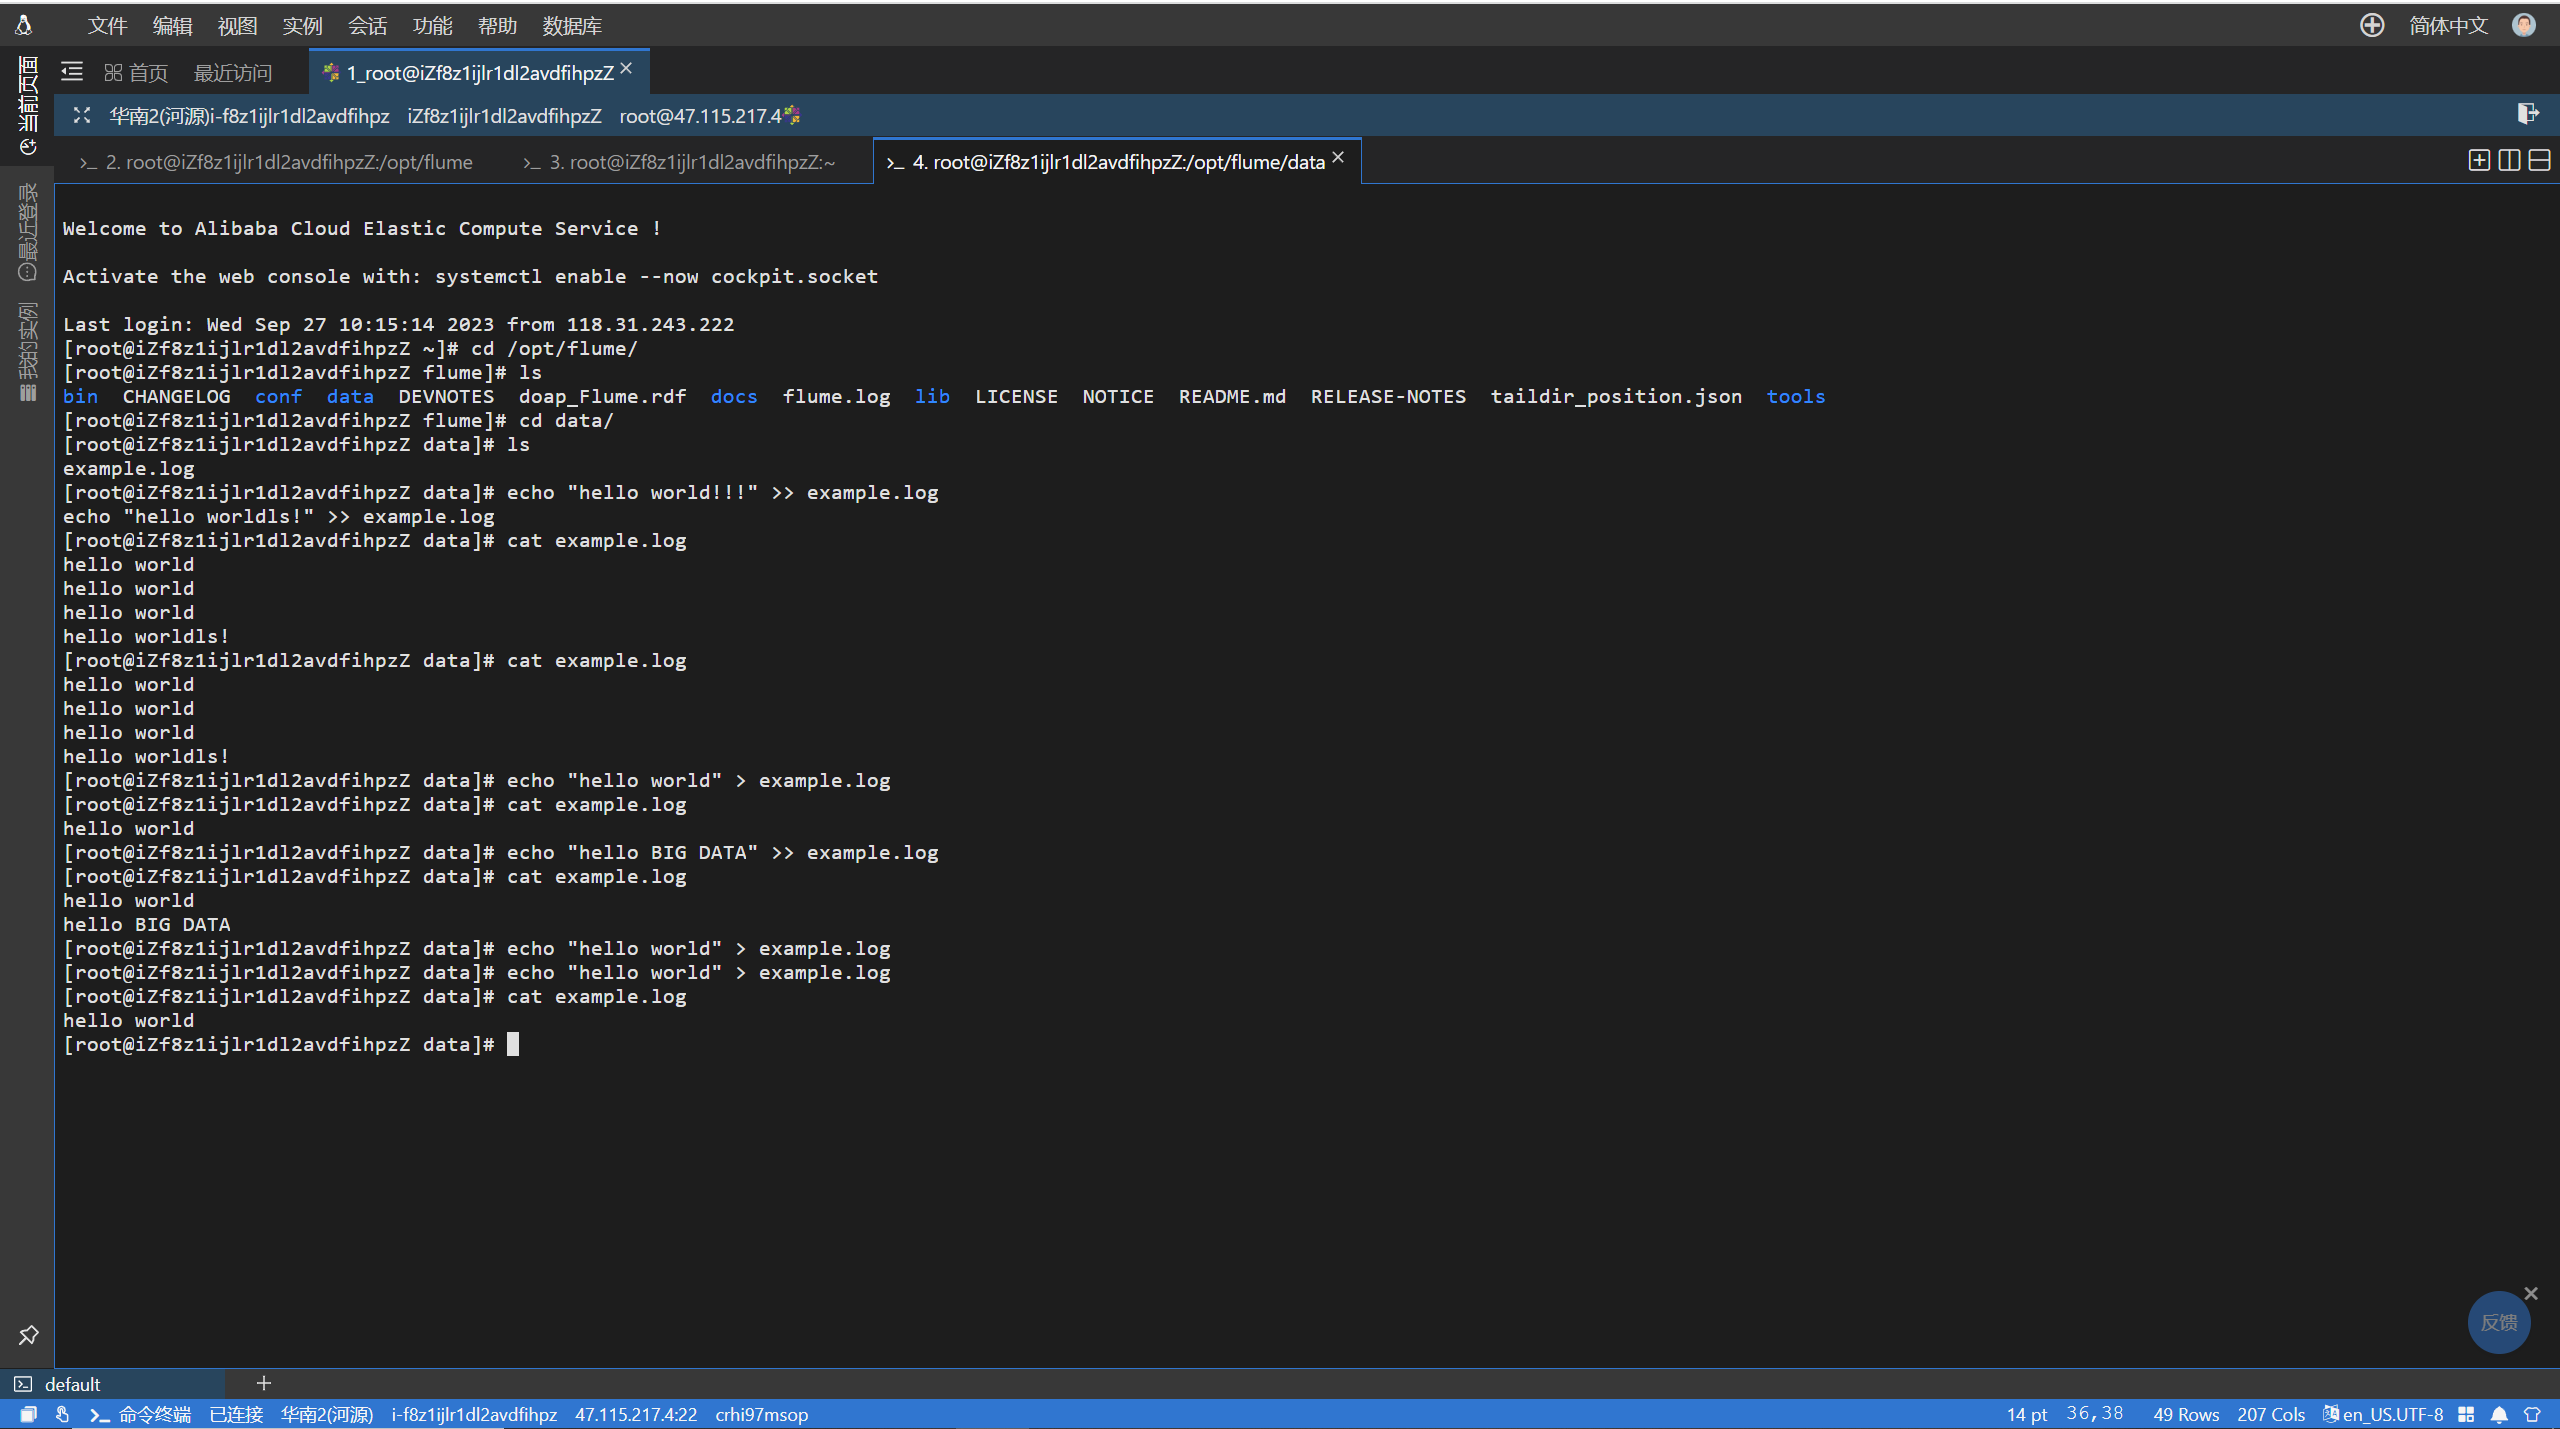
\includegraphics[width=15cm]{flume_inputToLog.png}
        \caption{flume 向example中输入}
        \label{pic6}
    \end{figure}
    \begin{lstlisting}
查看HDFS中保存的日志文件
hadoop fs -ls /flume/tailout/2023-09-27
    \end{lstlisting}
    \begin{figure}[htp]
        \centering
        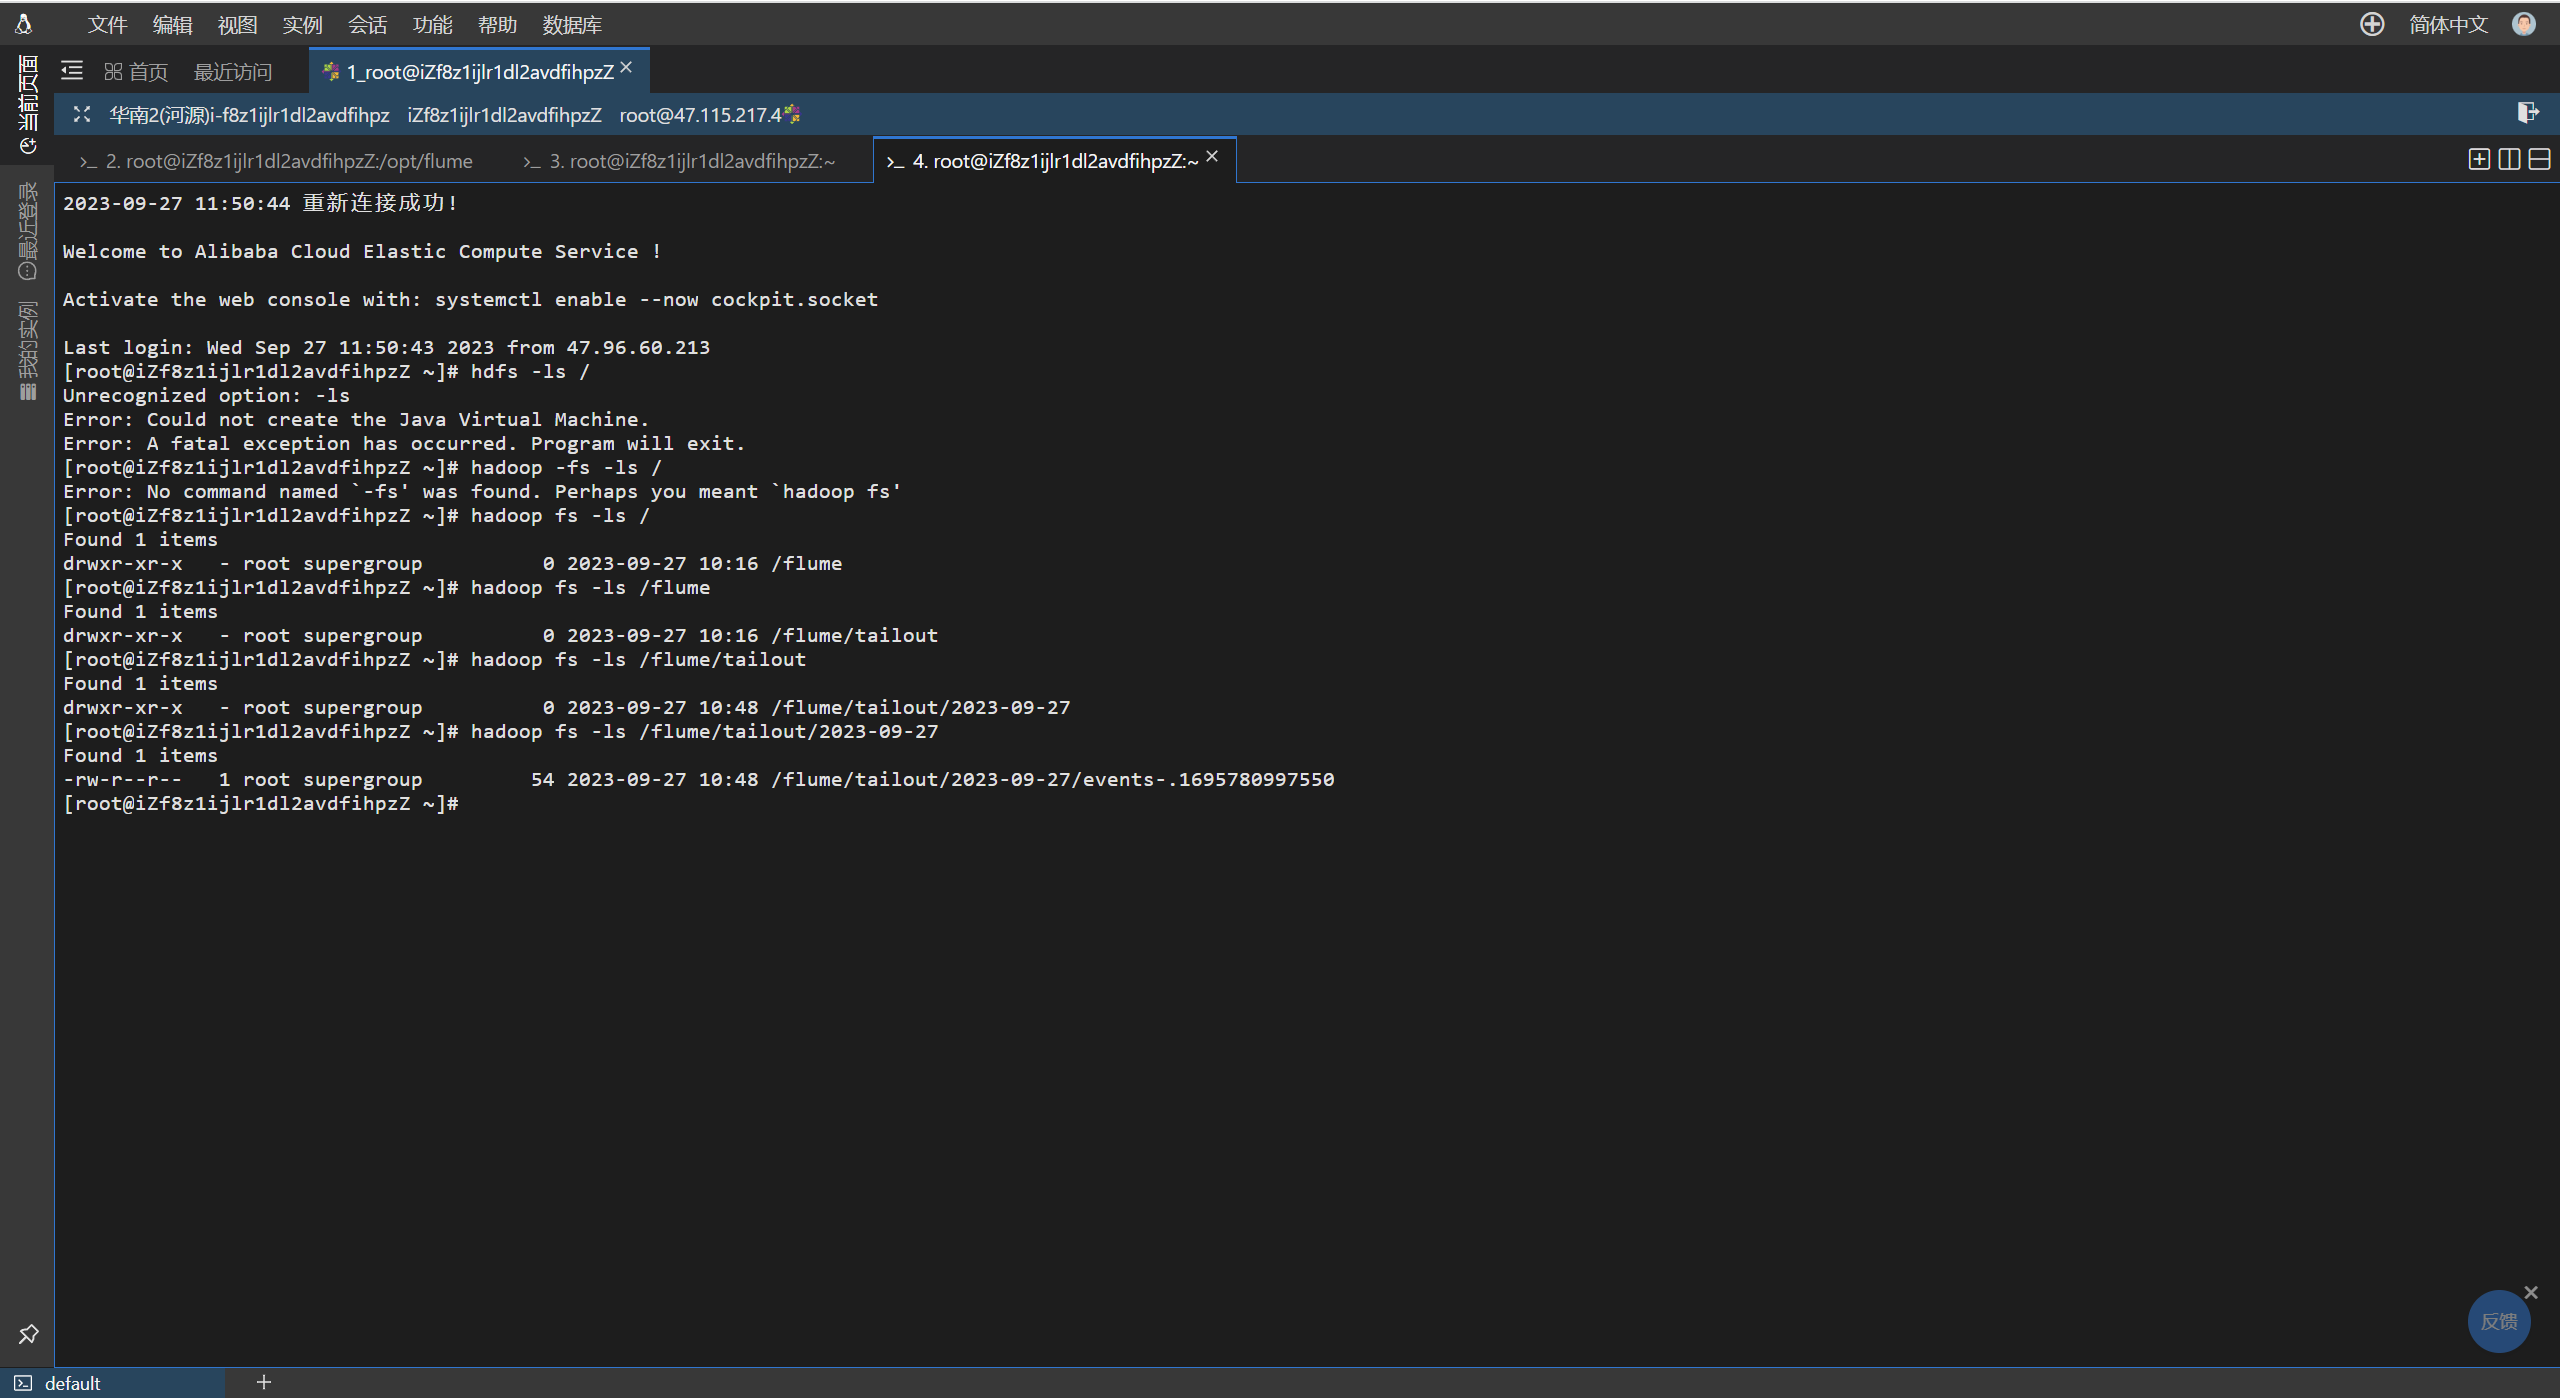
\includegraphics[width=15cm]{flume_hdfs.png}
        \caption{flume 查看hdfs中的日志文件}
        \label{pic7}
    \end{figure}
    \item 验证:确认 HDFS 中存储的日志
    \begin{figure}[htp]
        \centering
        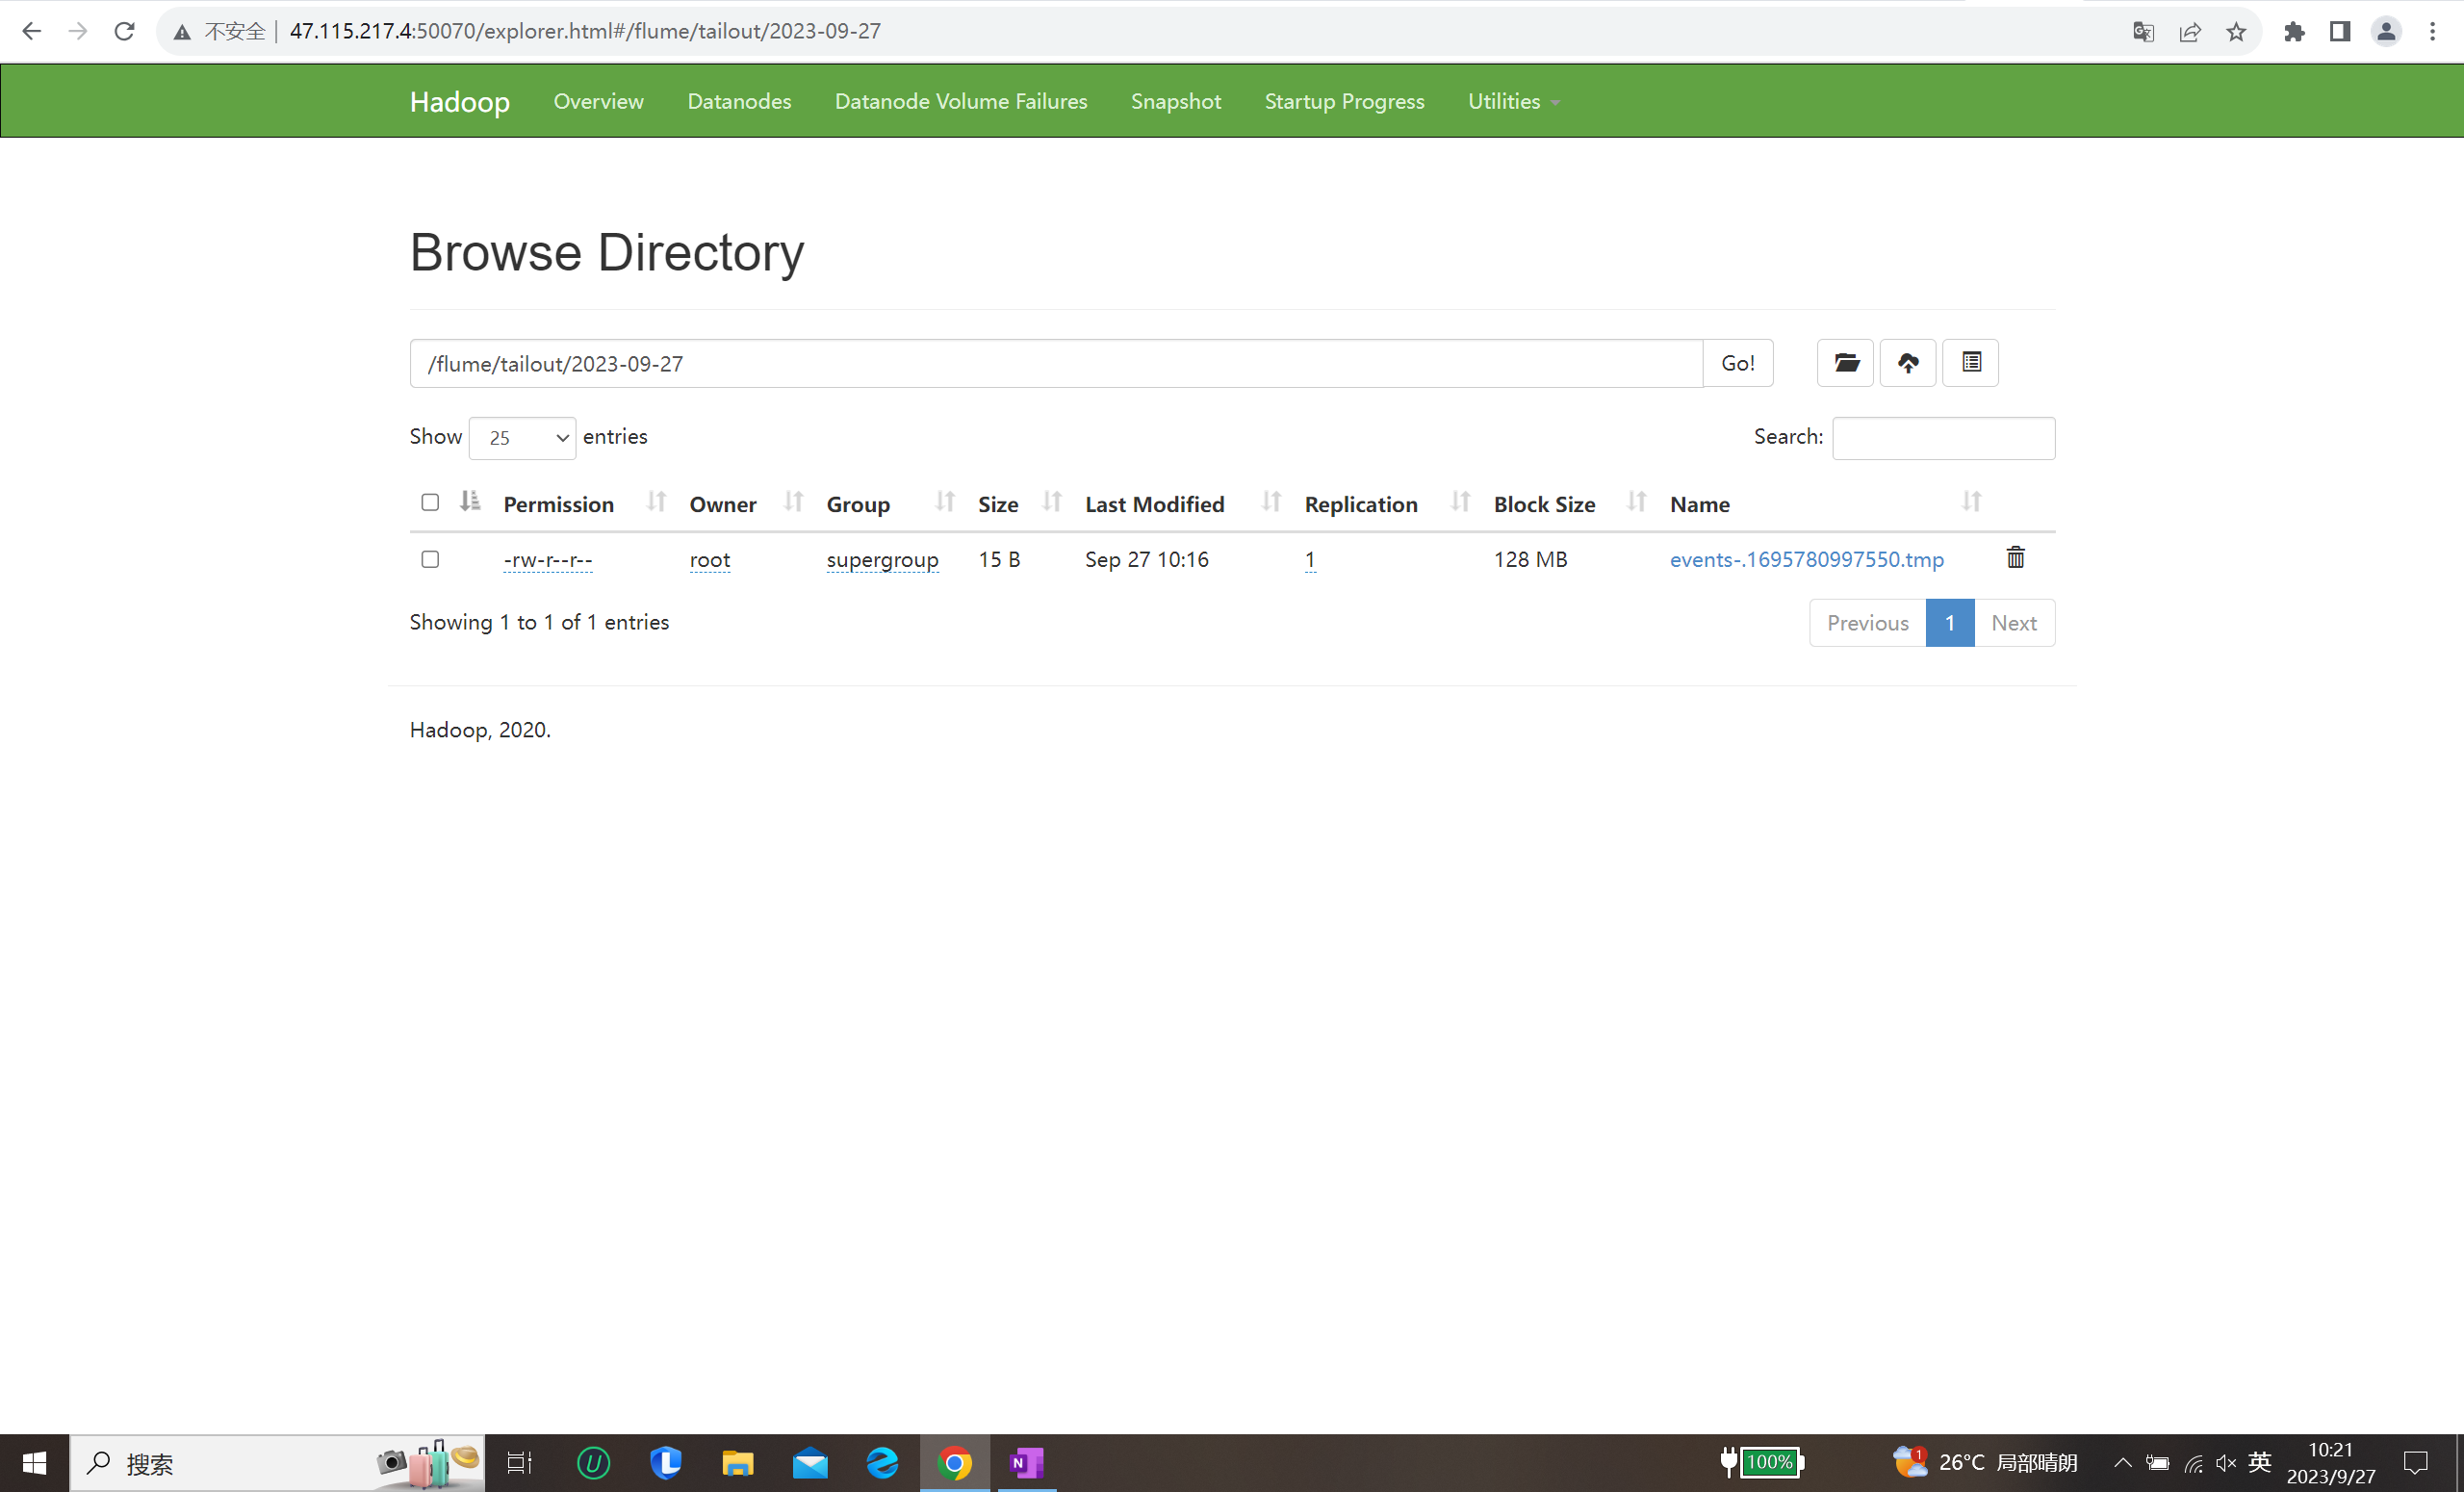
\includegraphics[width=15cm]{flume_logToHDFS.png}
        \caption{flume 查看hdfs中的日志文件}
        \label{pic8}
    \end{figure}
    

\end{enumerate}
\newpage
\section{过程中发现的困难及如何克服}
启动hadoop的时候:hadoop namenode -format命令又启动了一次,
结果namenode和datanode不能同时开启, 
上网查了很多资料, 最后删除了hadoop目录下的temp,
重新运行hadoop namenode -format就好了.



\end{document}
